\documentclass[UTF8,a4paper]{paper}
\usepackage[utf8]{inputenc}
\usepackage{ctex}
\usepackage{amsmath}
\usepackage{pdfpages}
\usepackage{graphicx}
\usepackage{wrapfig}
\usepackage{listings}
\usepackage{multicol}
\usepackage{float}
\title{第三次仿真实验报告}
\author{张蔚桐\ 2015011493\ 自55}
\begin {document}
\newcommand{\tabincell}[2]{\begin{tabular}{@{}#1@{}}#2\end{tabular}}
\maketitle
\tableofcontents
\clearpage
\section{一阶微分方程求解电路}
\begin{figure}
\centering
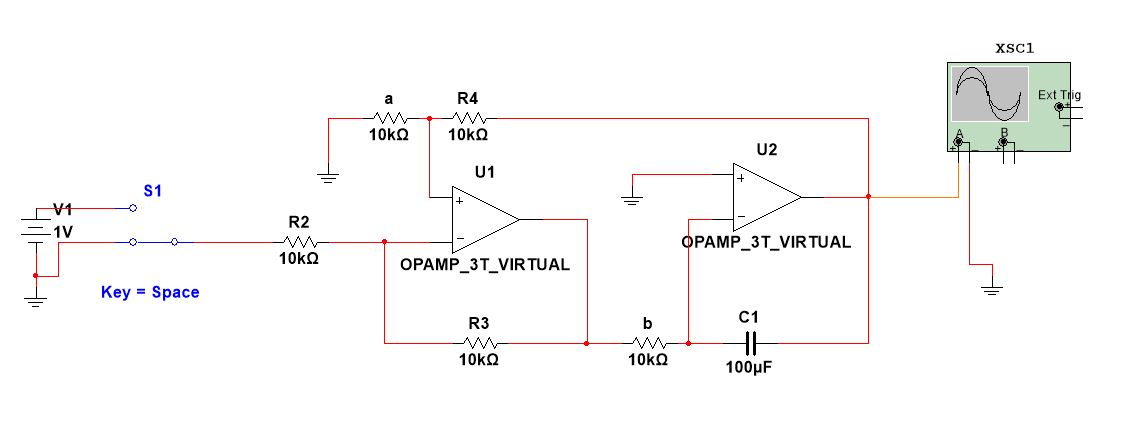
\includegraphics[width=\textwidth]{cir1.jpg}
\caption{求解一阶微分方程的运算电路}
\label{cir1}
\end{figure}
\section{VCVS电路搭建和测试}
\subsection{辐频相频特性的测量}
\subsubsection{VCVS低通滤波电路搭建和测试}
\begin{figure}
\centering
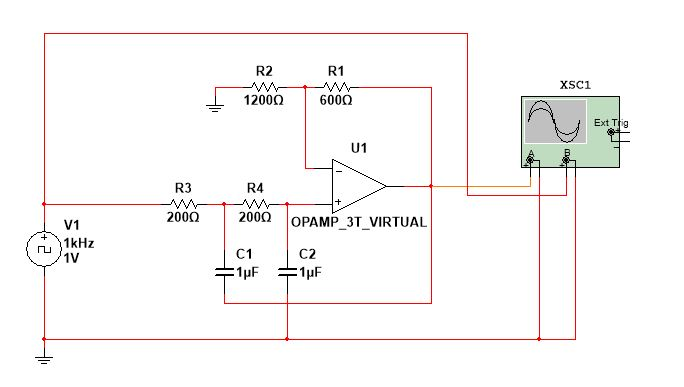
\includegraphics[width=\textwidth]{L.jpg}
\caption{VCVS低通滤波电路}
\label{L}
\end{figure}
\begin{figure}
\centering
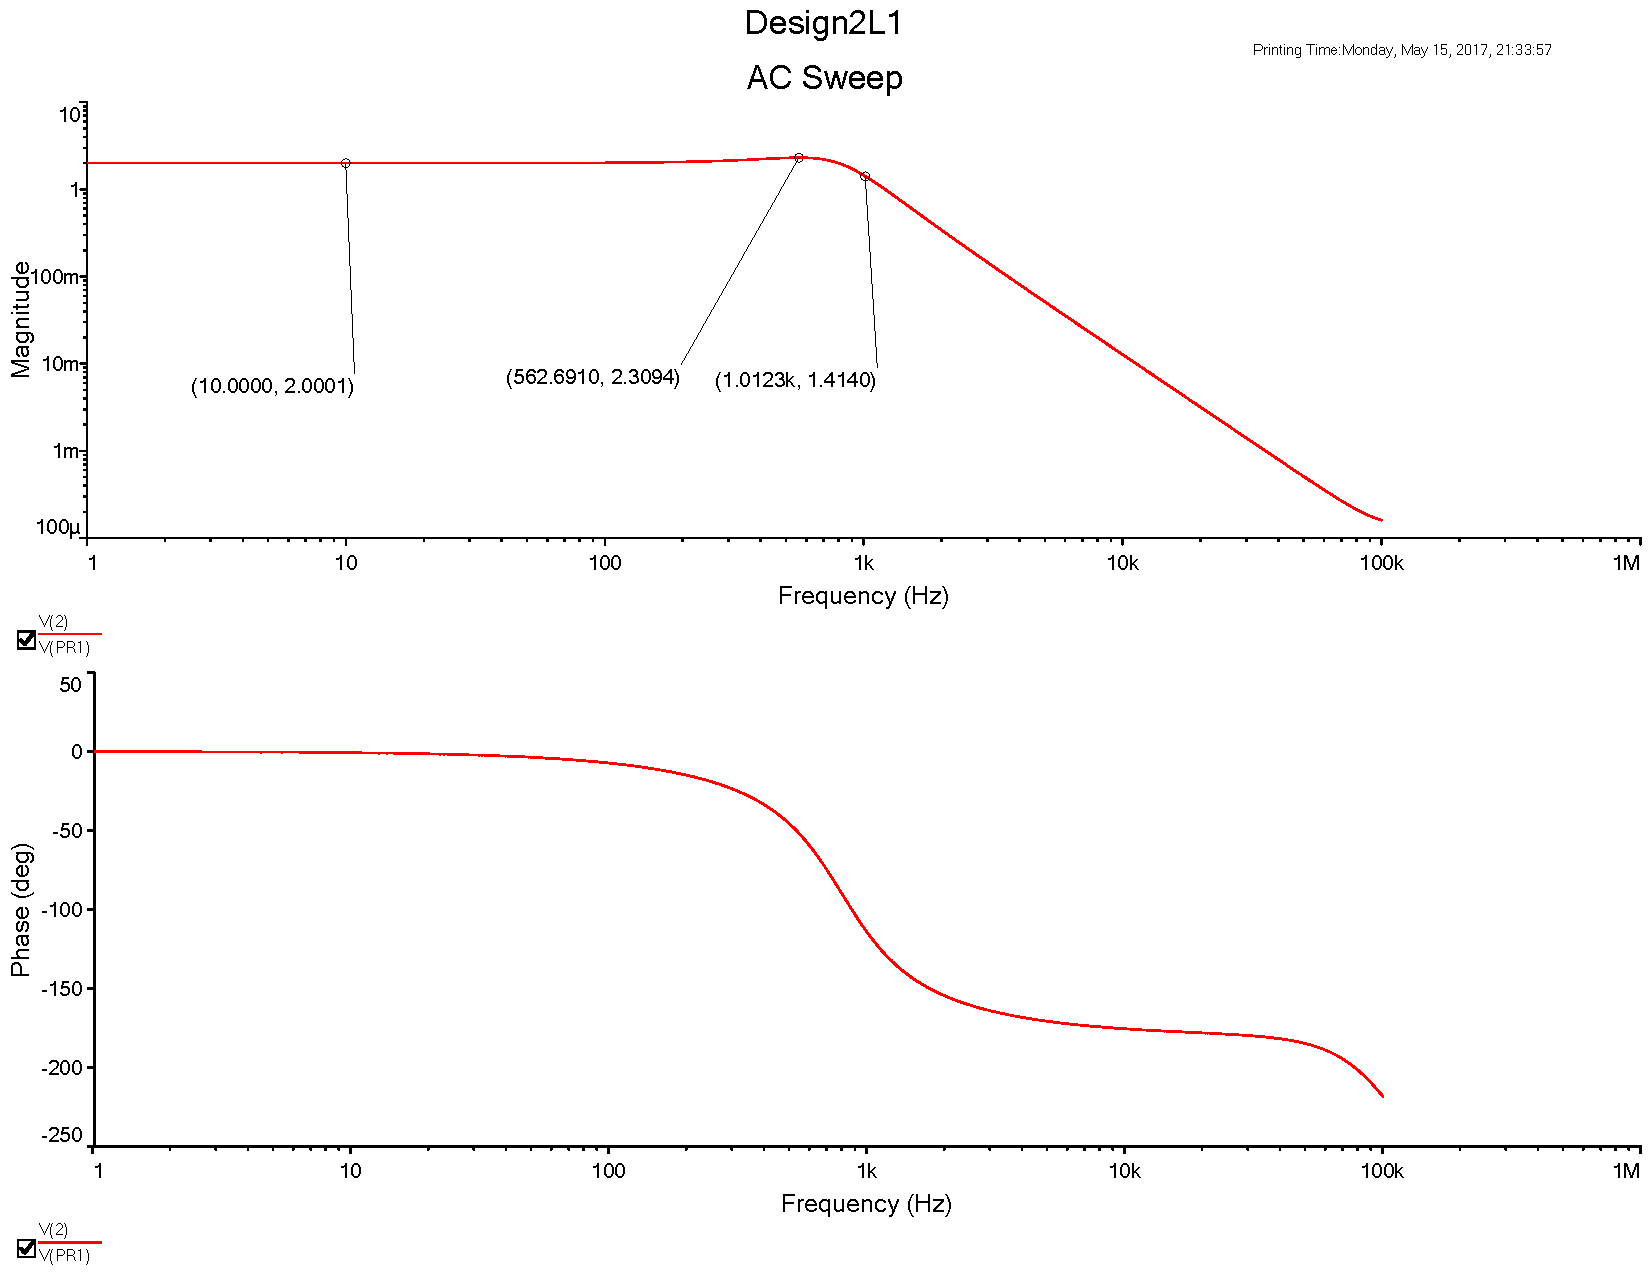
\includegraphics[width=\textwidth]{2L1.pdf}
\caption{Q=1}
\label{LQ1}
\end{figure}
\begin{figure}
\centering
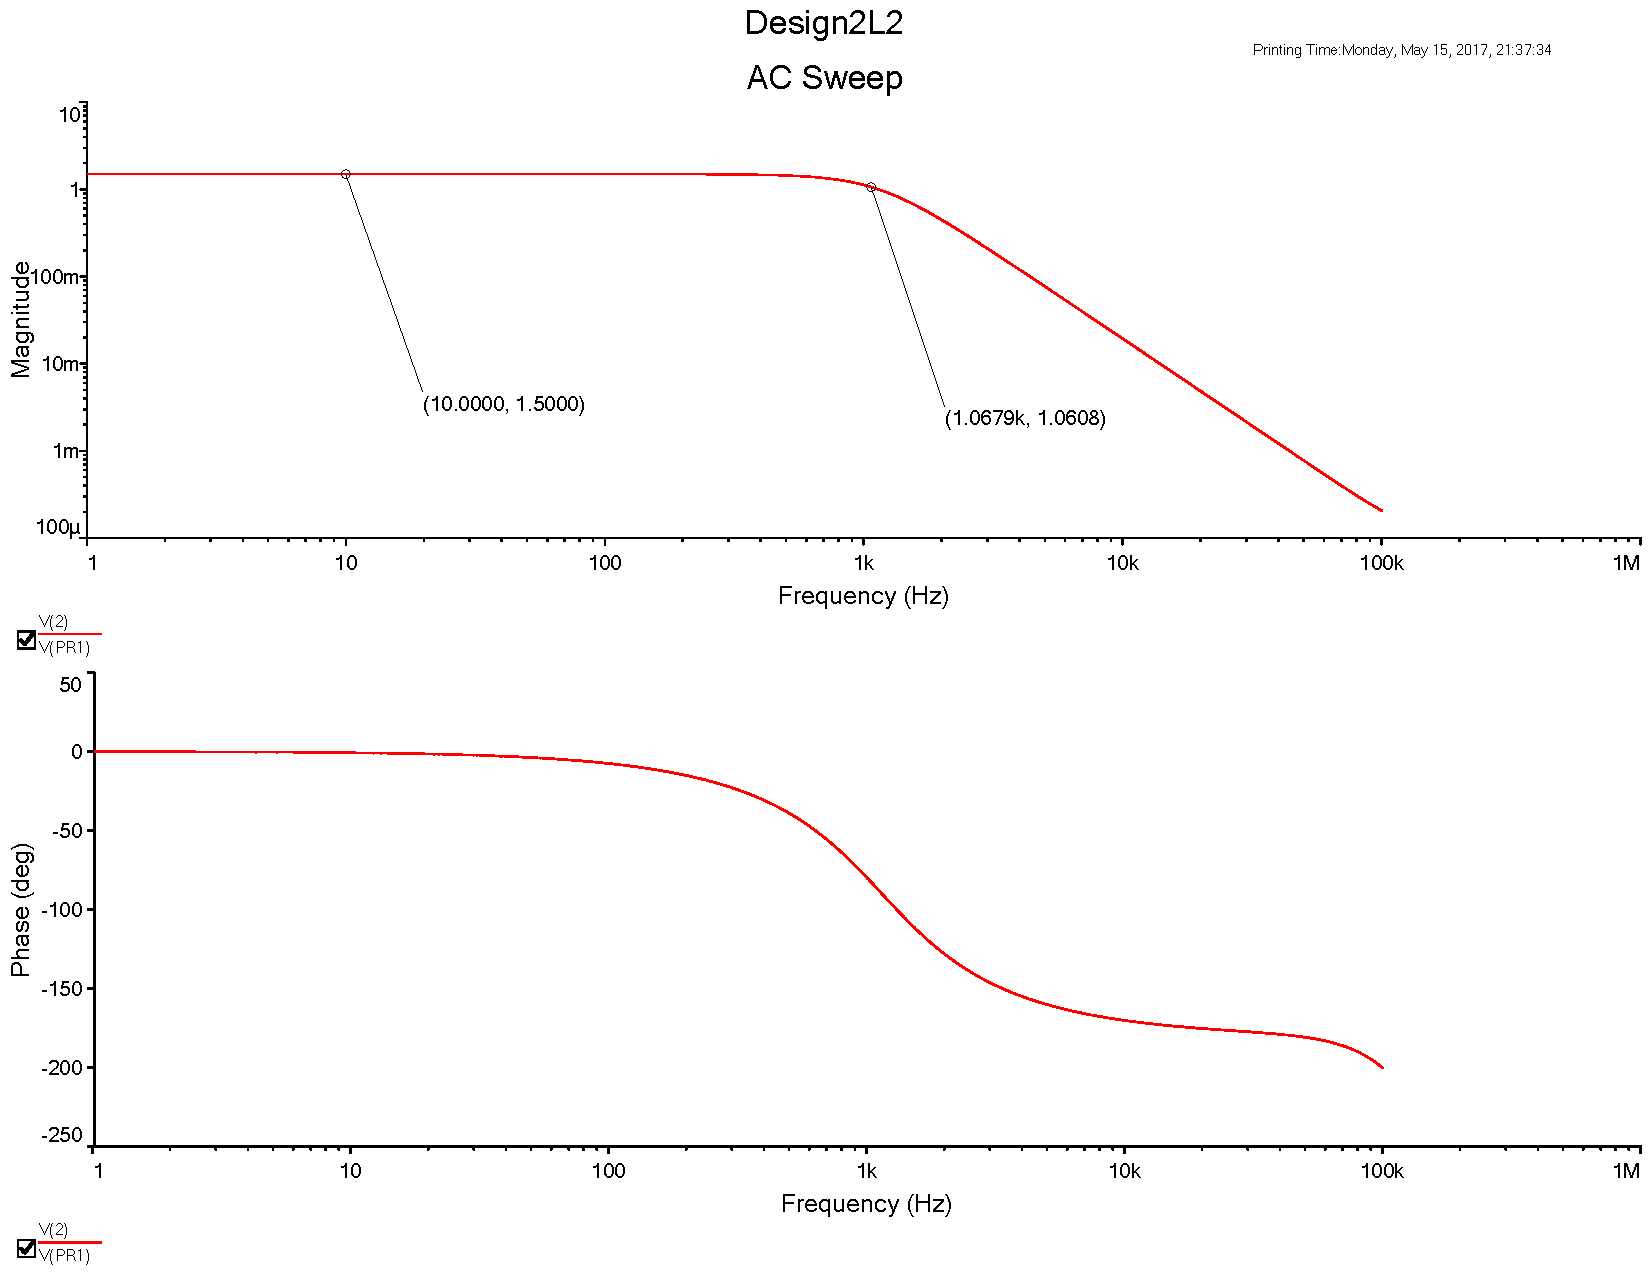
\includegraphics[width=\textwidth]{2L2_3.pdf}
\caption{$Q=2/3$}
\label{LQ23}
\end{figure}
\begin{figure}
\centering
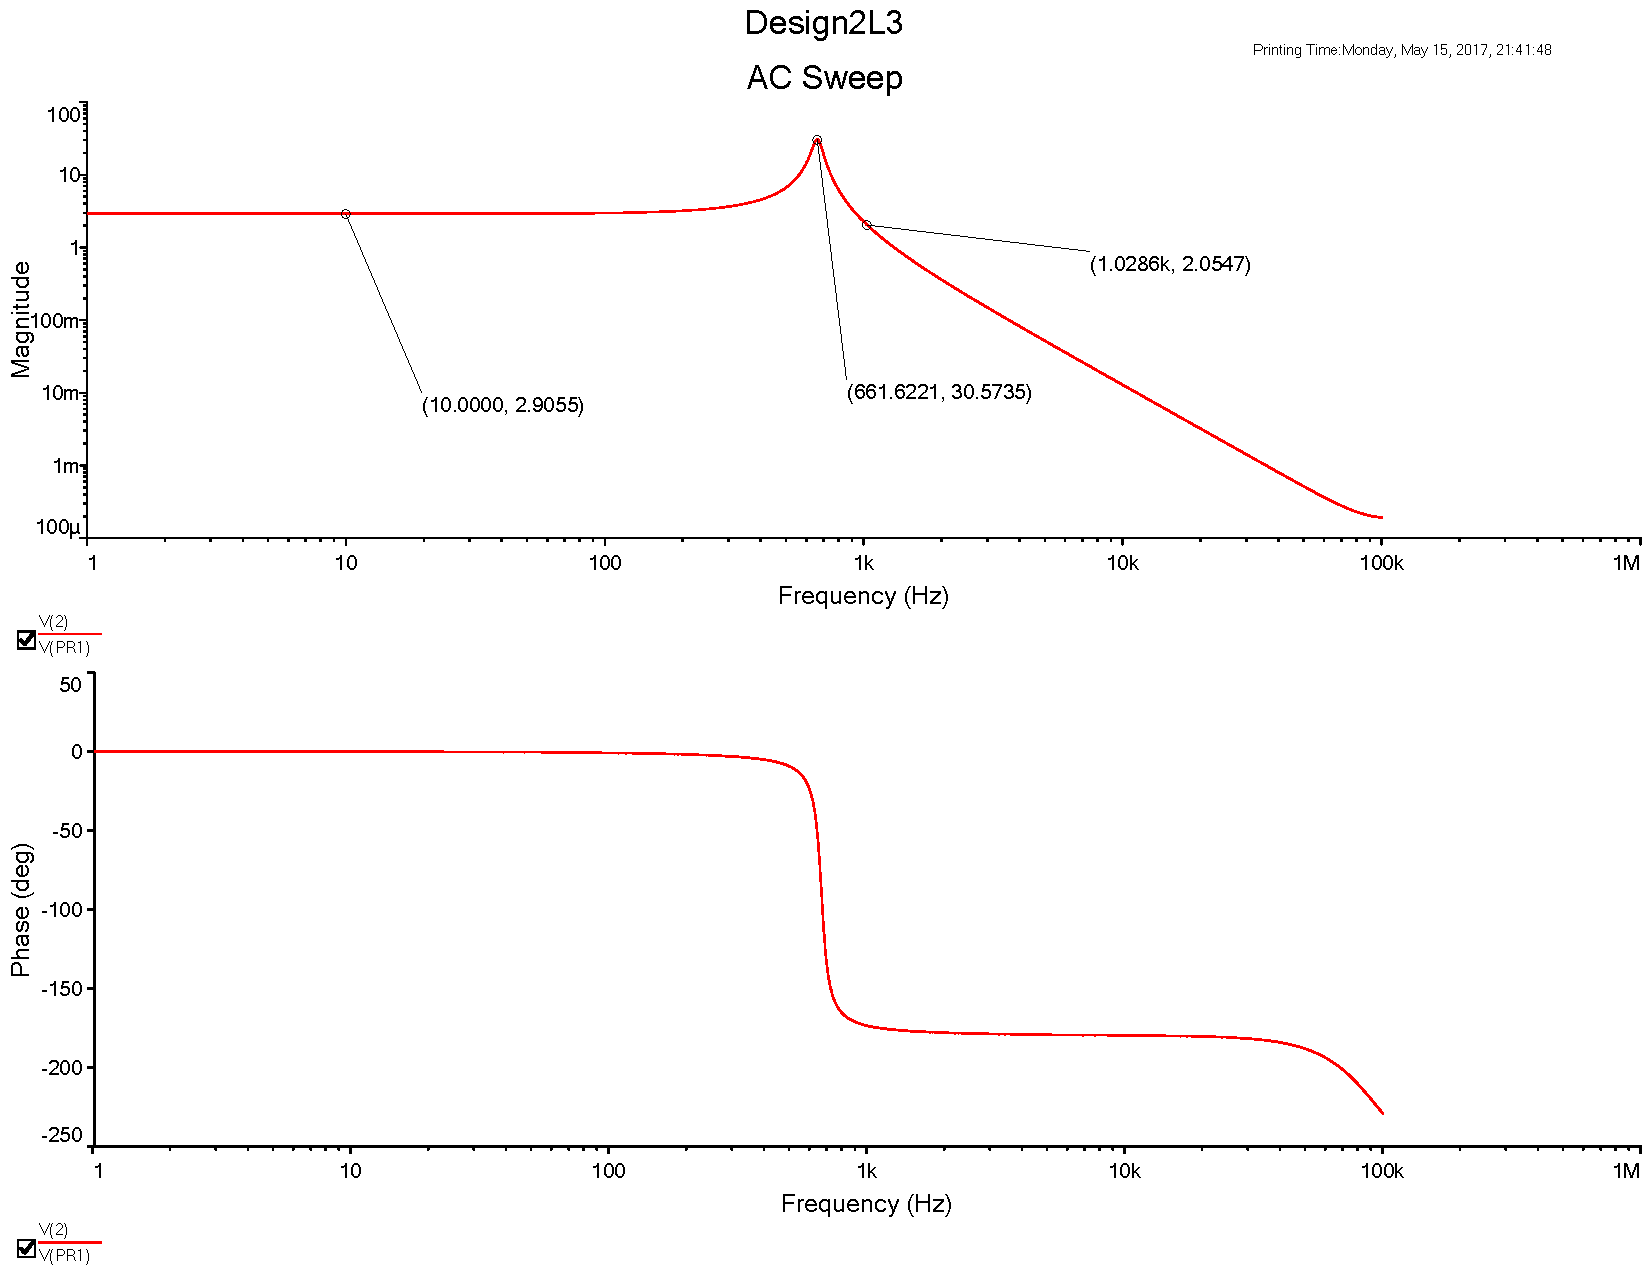
\includegraphics[width=\textwidth]{2L10_5.pdf}
\caption{$Q=10.5$}
\label{LQ10}
\end{figure}
\clearpage
\subsubsection{VCVS高通滤波电路搭建和测试}
\begin{figure}
\centering
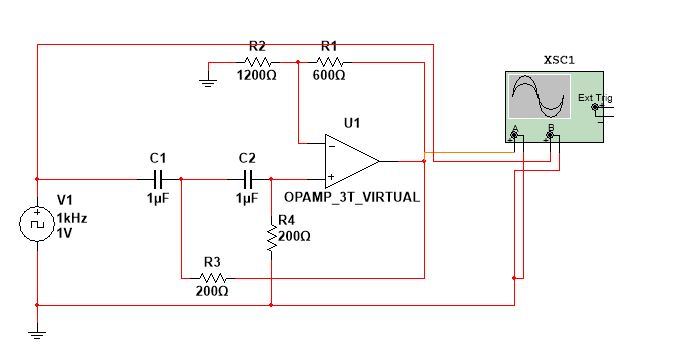
\includegraphics[width=\textwidth]{H.jpg}
\caption{VCVS高通滤波电路}
\label{H}
\end{figure}
\begin{figure}
\centering
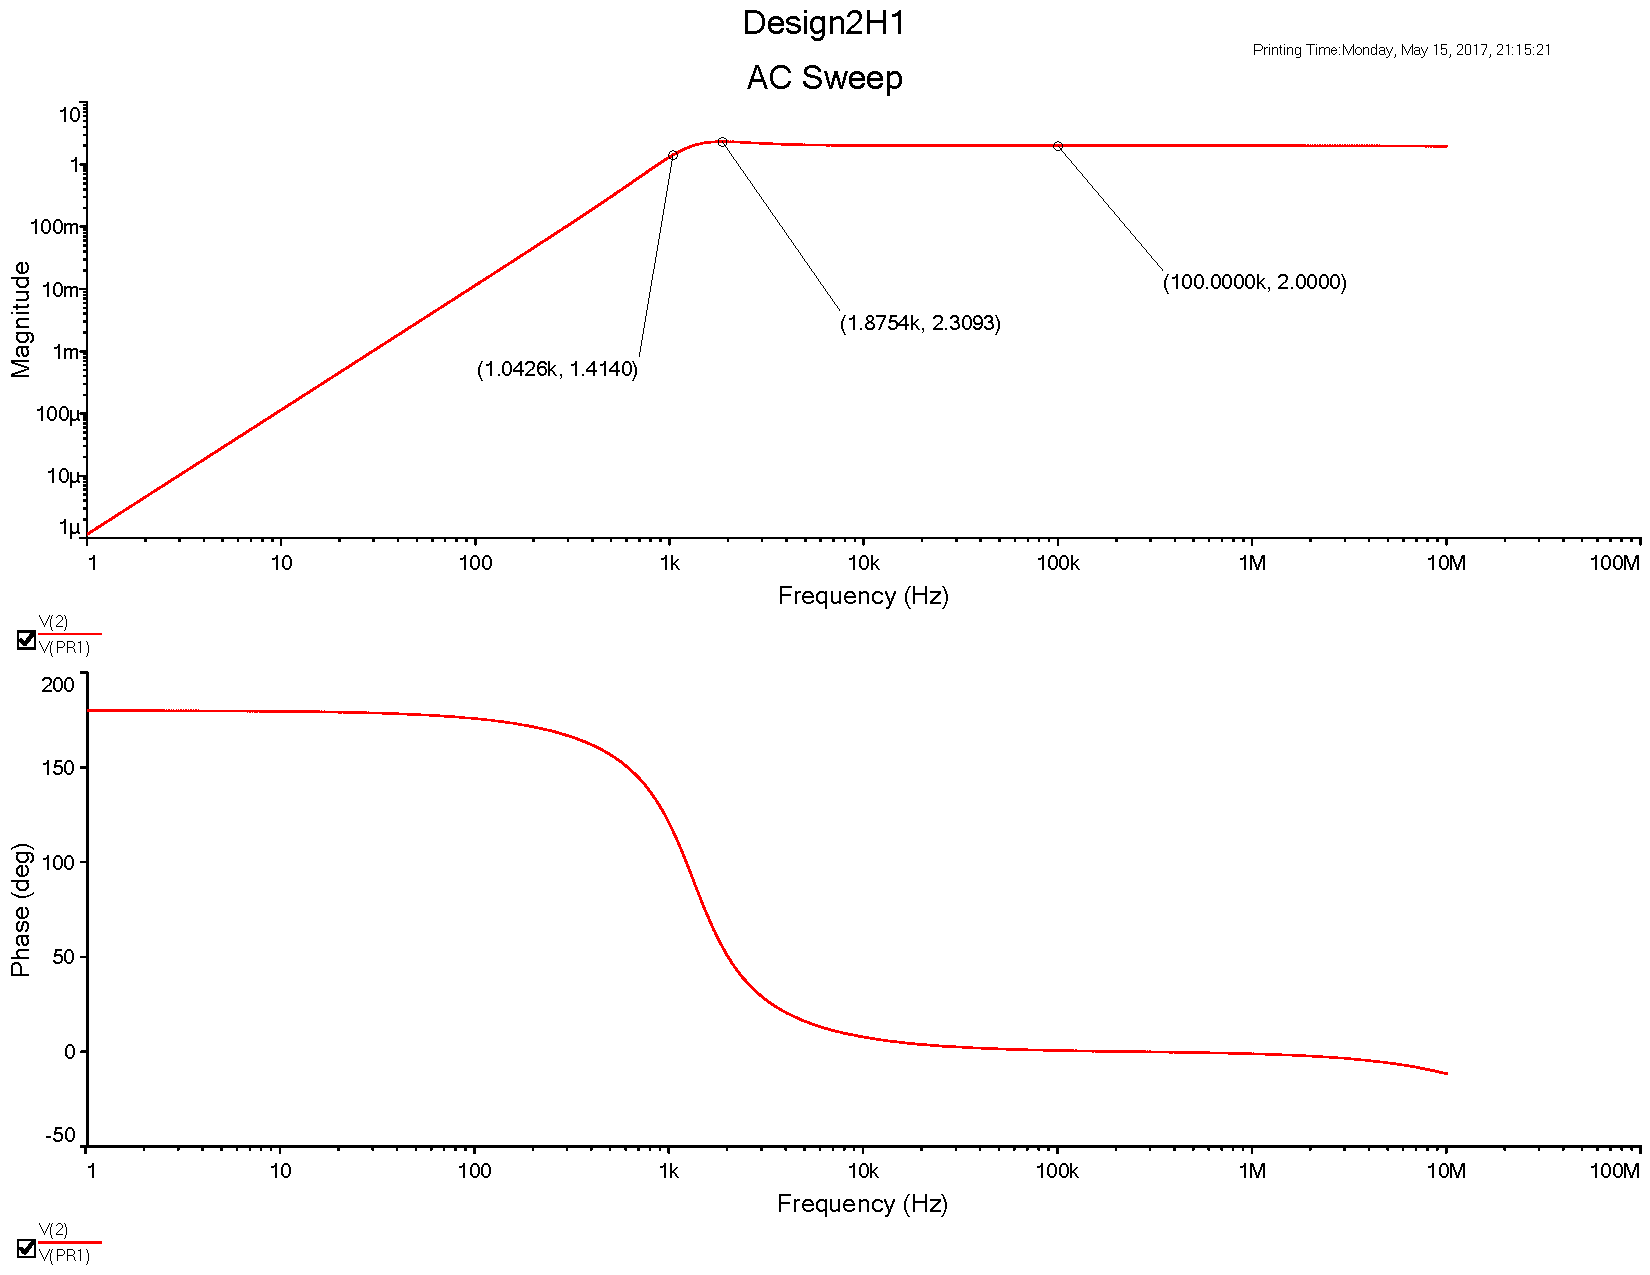
\includegraphics[width=\textwidth]{2H1.pdf}
\caption{Q=1}
\label{HQ1}
\end{figure}
\begin{figure}
\centering
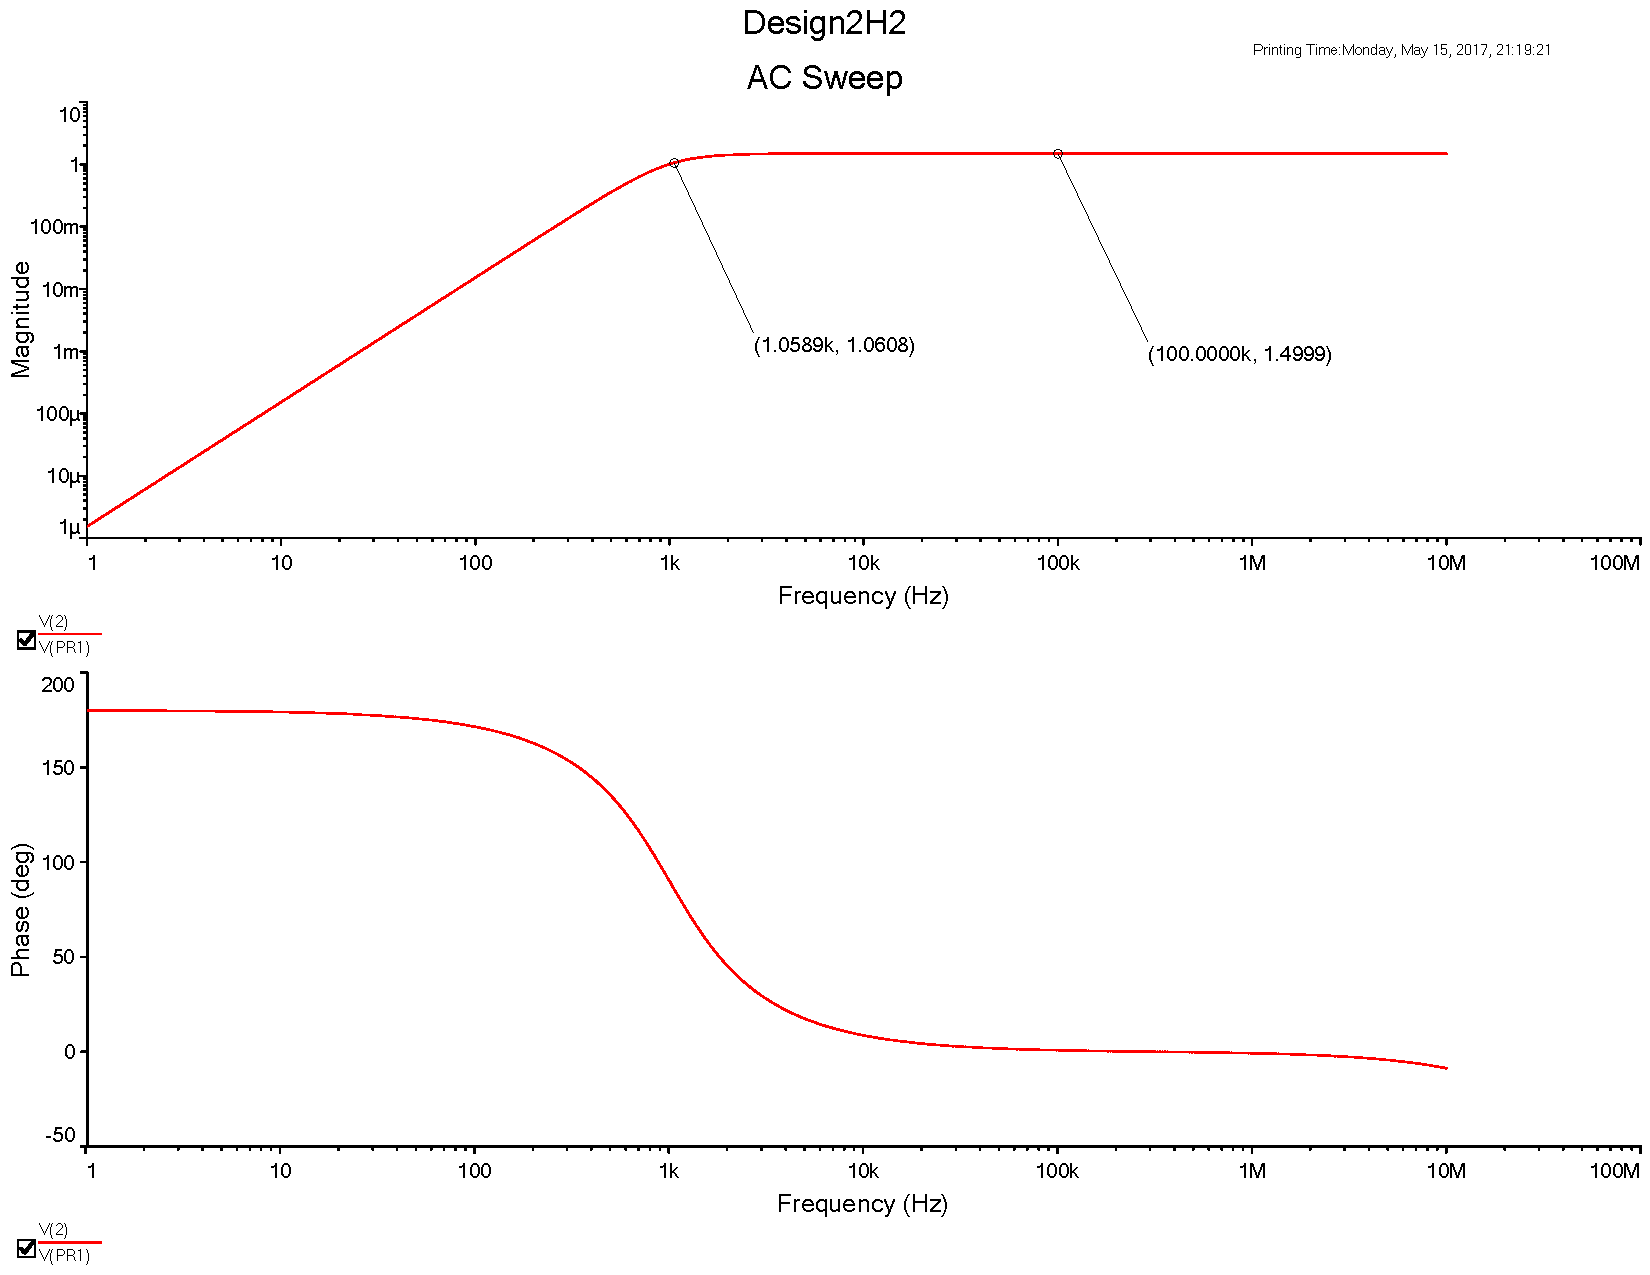
\includegraphics[width=\textwidth]{2H2_3.pdf}
\caption{$Q=2/3$}
\label{HQ23}
\end{figure}
\begin{figure}
\centering
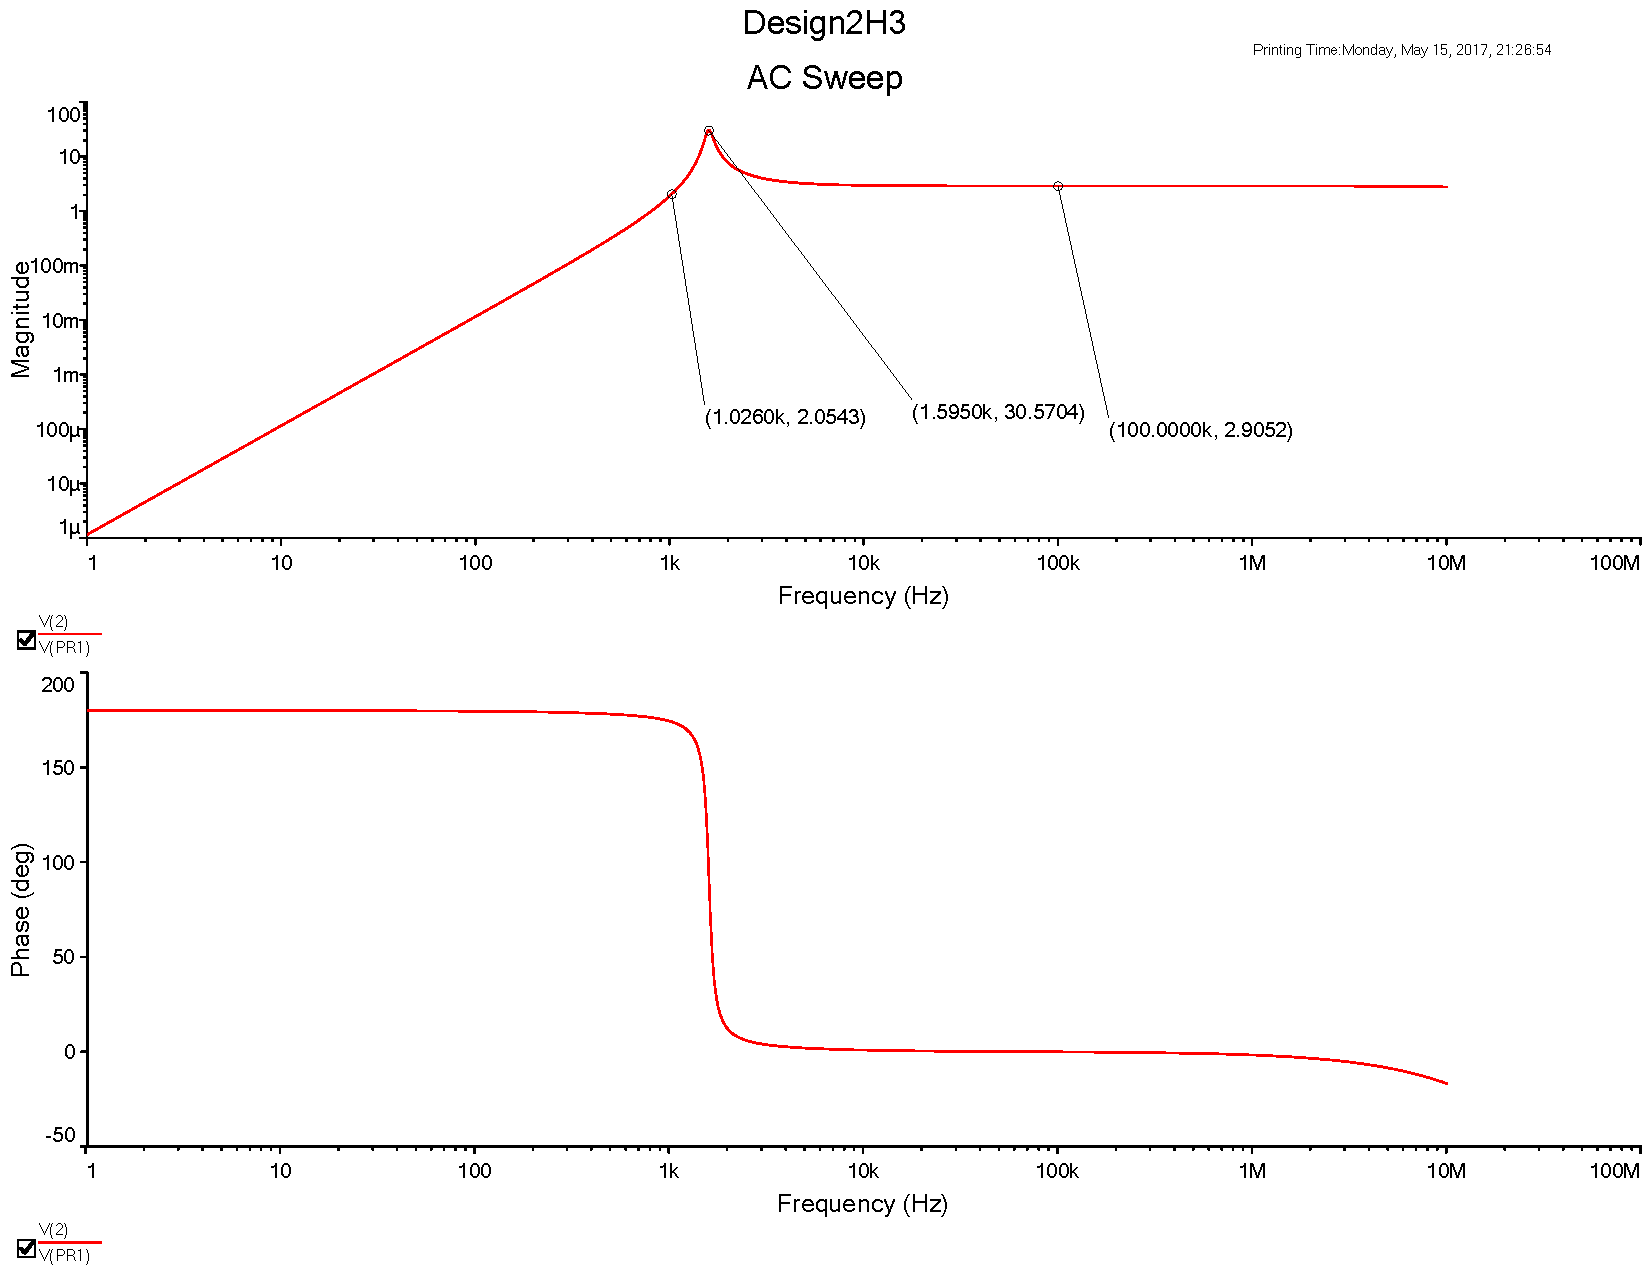
\includegraphics[width=\textwidth]{2H10_5.pdf}
\caption{$Q=10.5$}
\label{HQ10}
\end{figure}
\clearpage
\subsubsection{VCVS带通滤波电路搭建和测试}
\begin{figure}
\centering
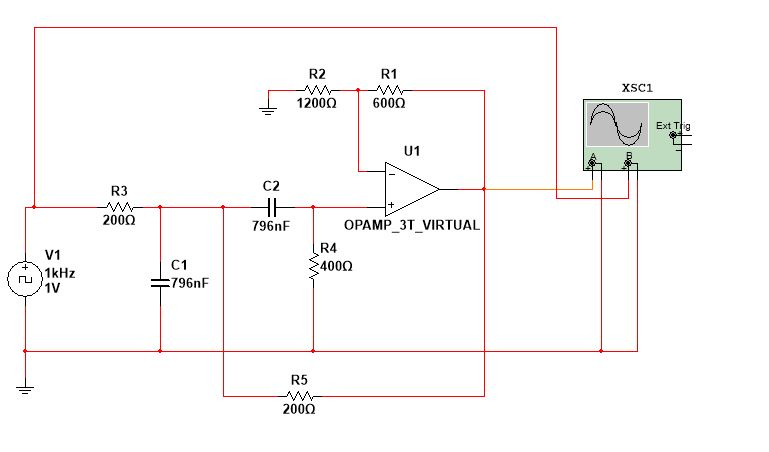
\includegraphics[width=\textwidth]{P.jpg}
\caption{VCVS带通滤波电路}
\label{P}
\end{figure}
\begin{figure}
\centering
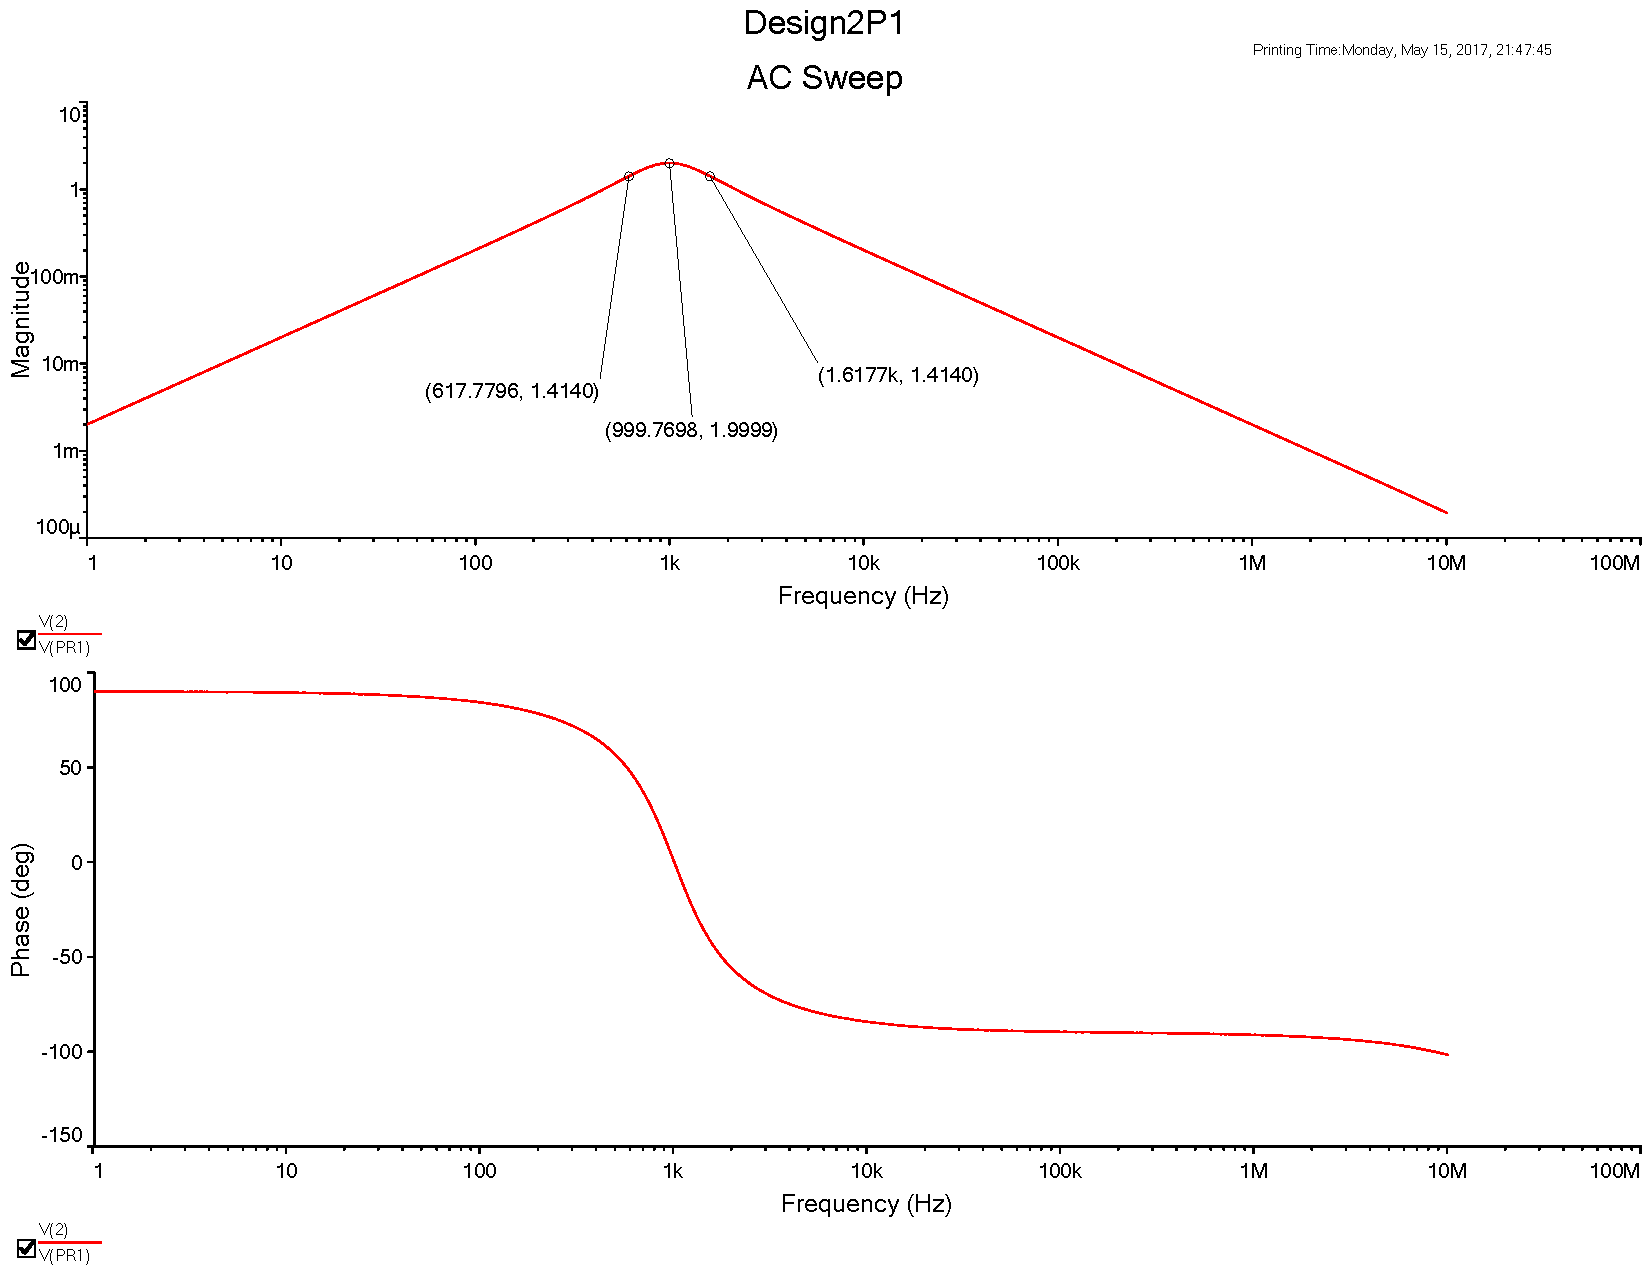
\includegraphics[width=\textwidth]{2P1.pdf}
\caption{Q=1}
\label{LQ1}
\end{figure}
\begin{figure}
\centering
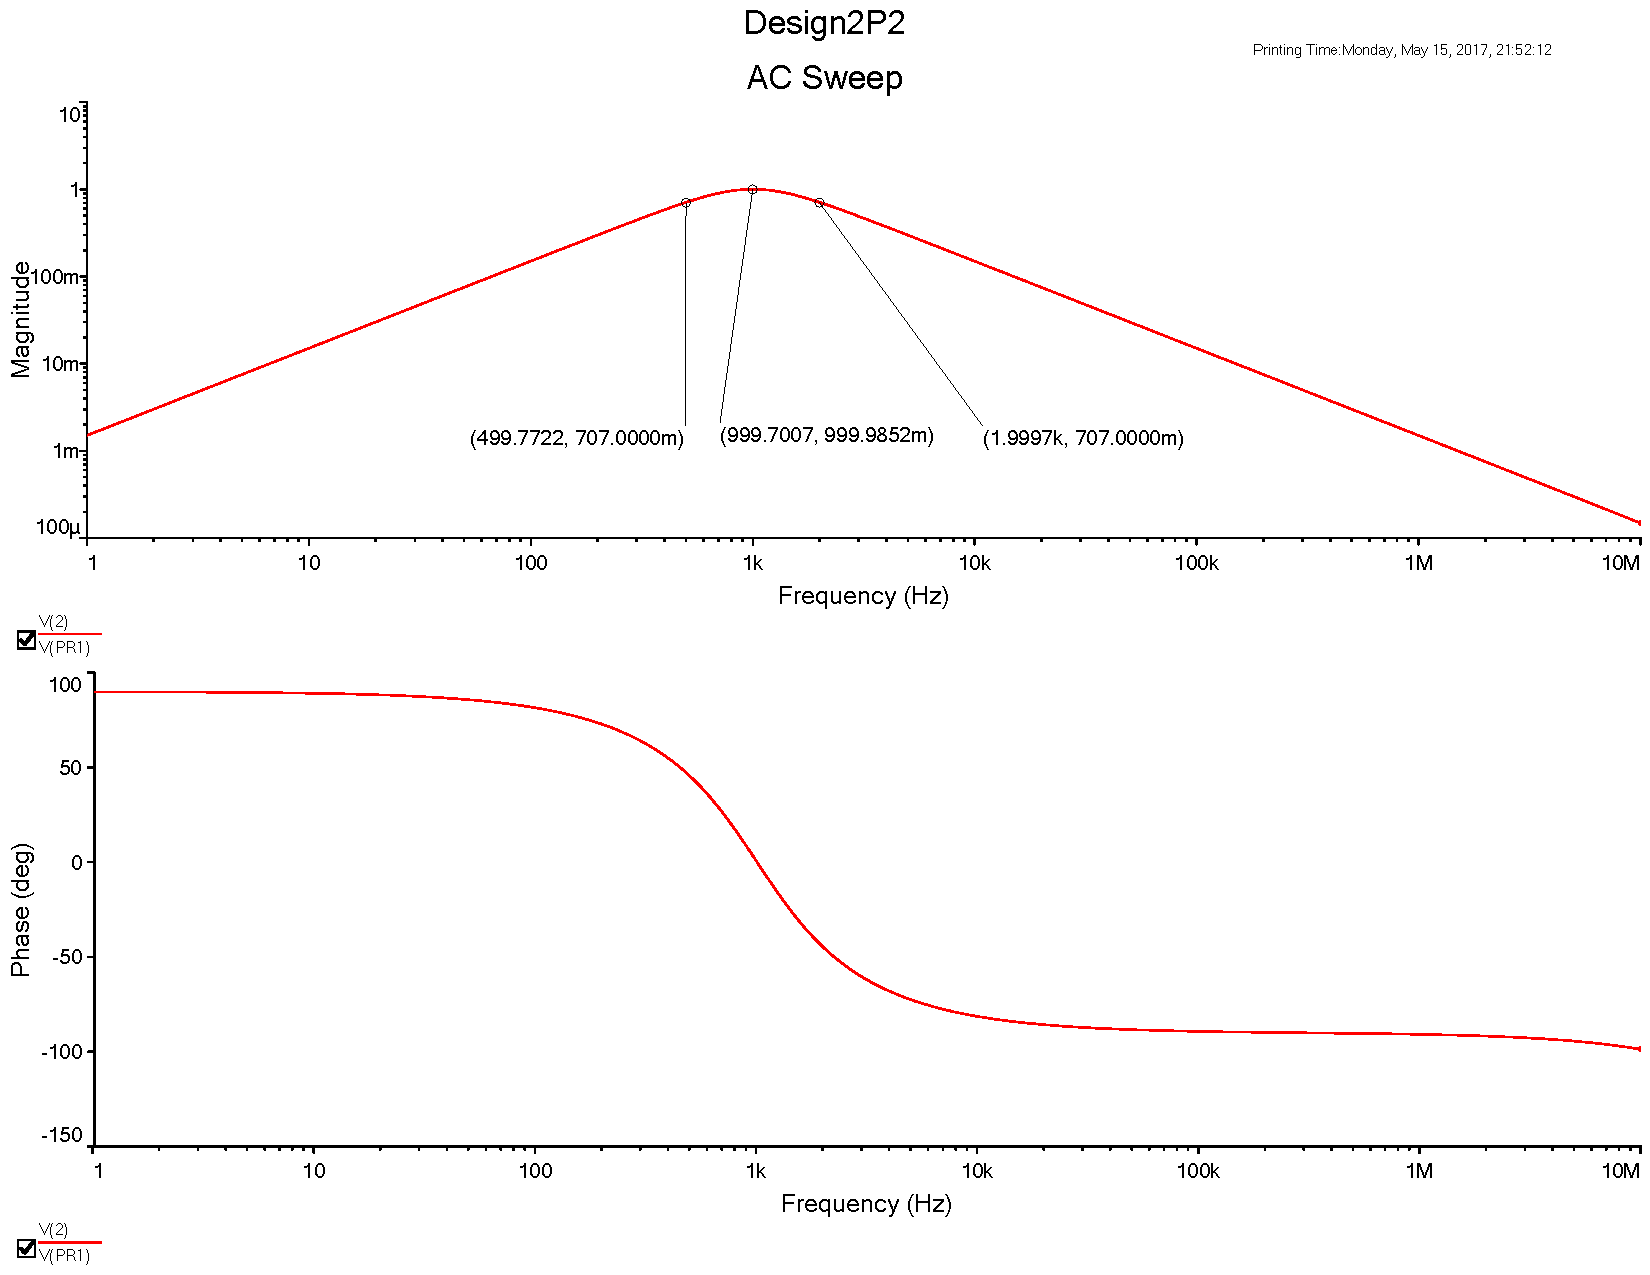
\includegraphics[width=\textwidth]{2P2_3.pdf}
\caption{$Q=2/3$}
\label{PQ23}
\end{figure}
\begin{figure}
\centering
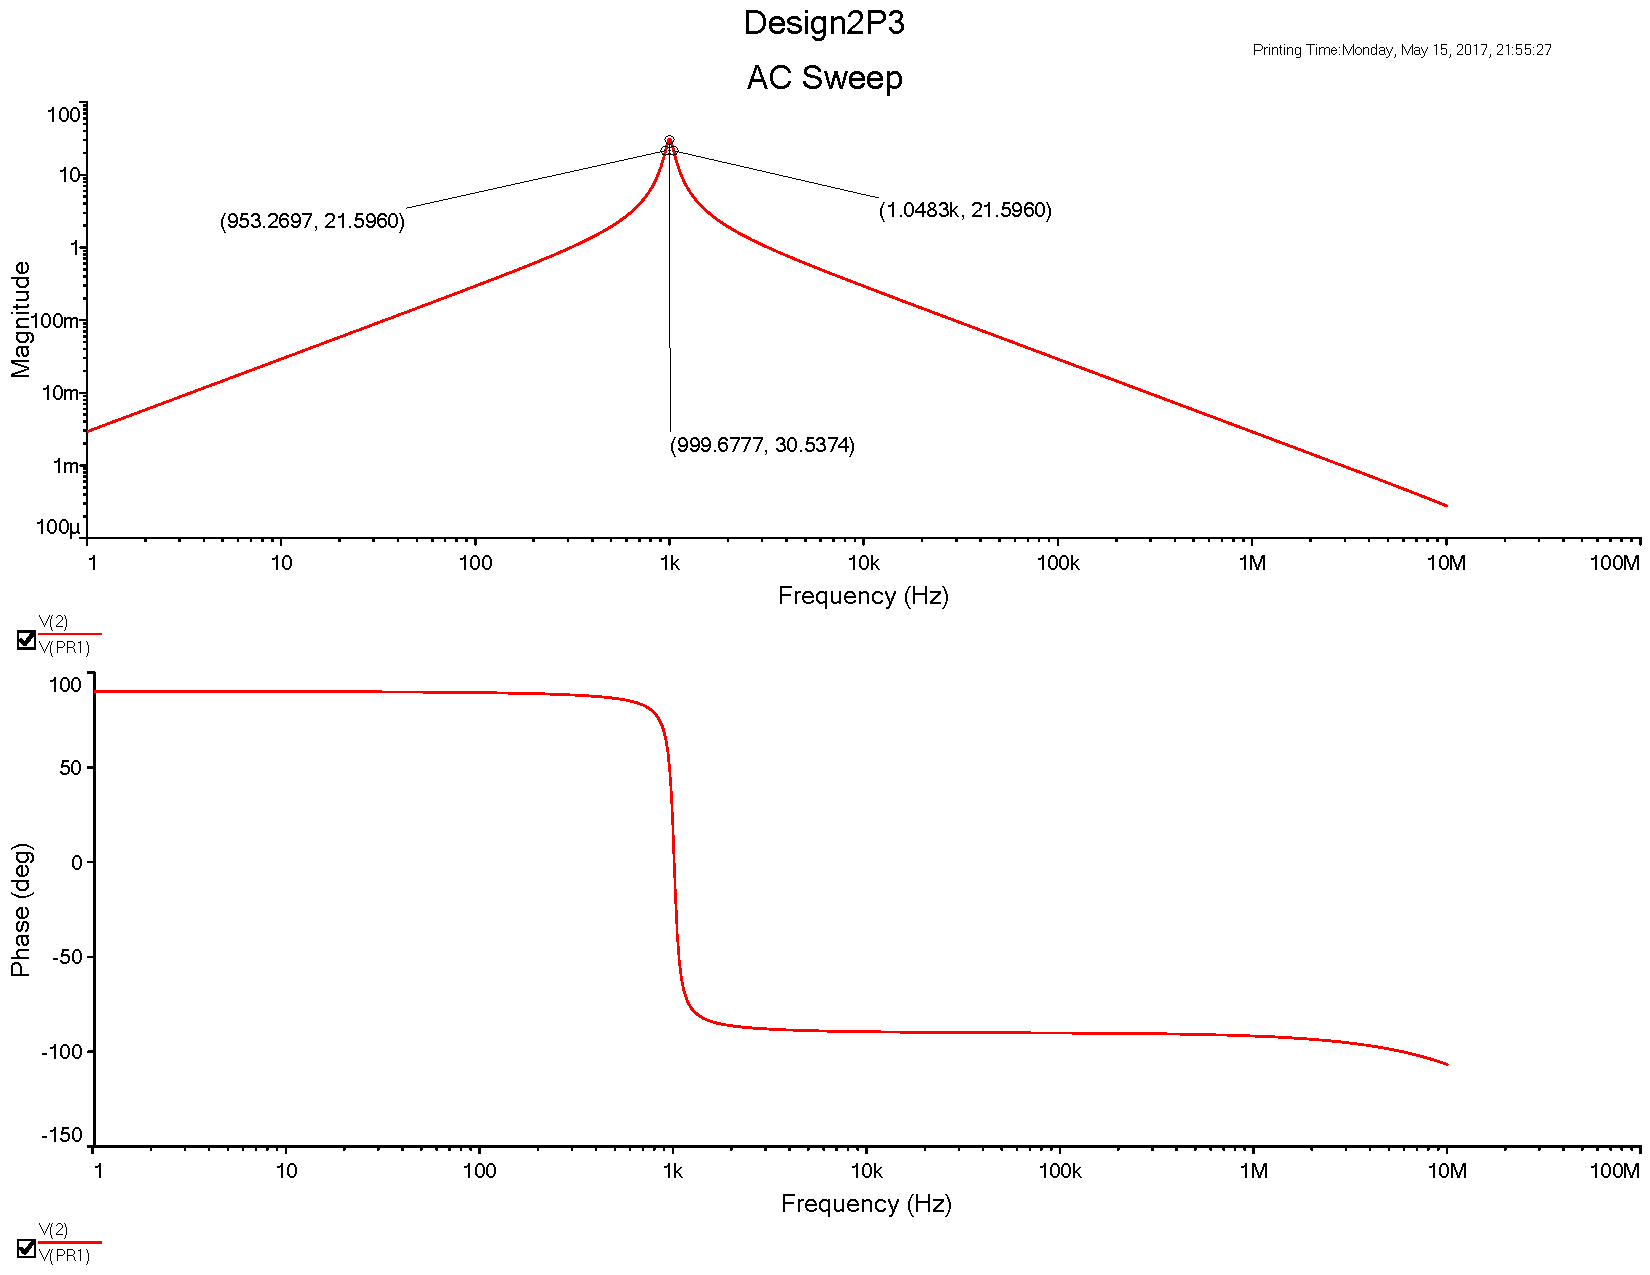
\includegraphics[width=\textwidth]{2P10_5.pdf}
\caption{$Q=10.5$}
\label{PQ10}
\end{figure}
\begin{figure}
\centering
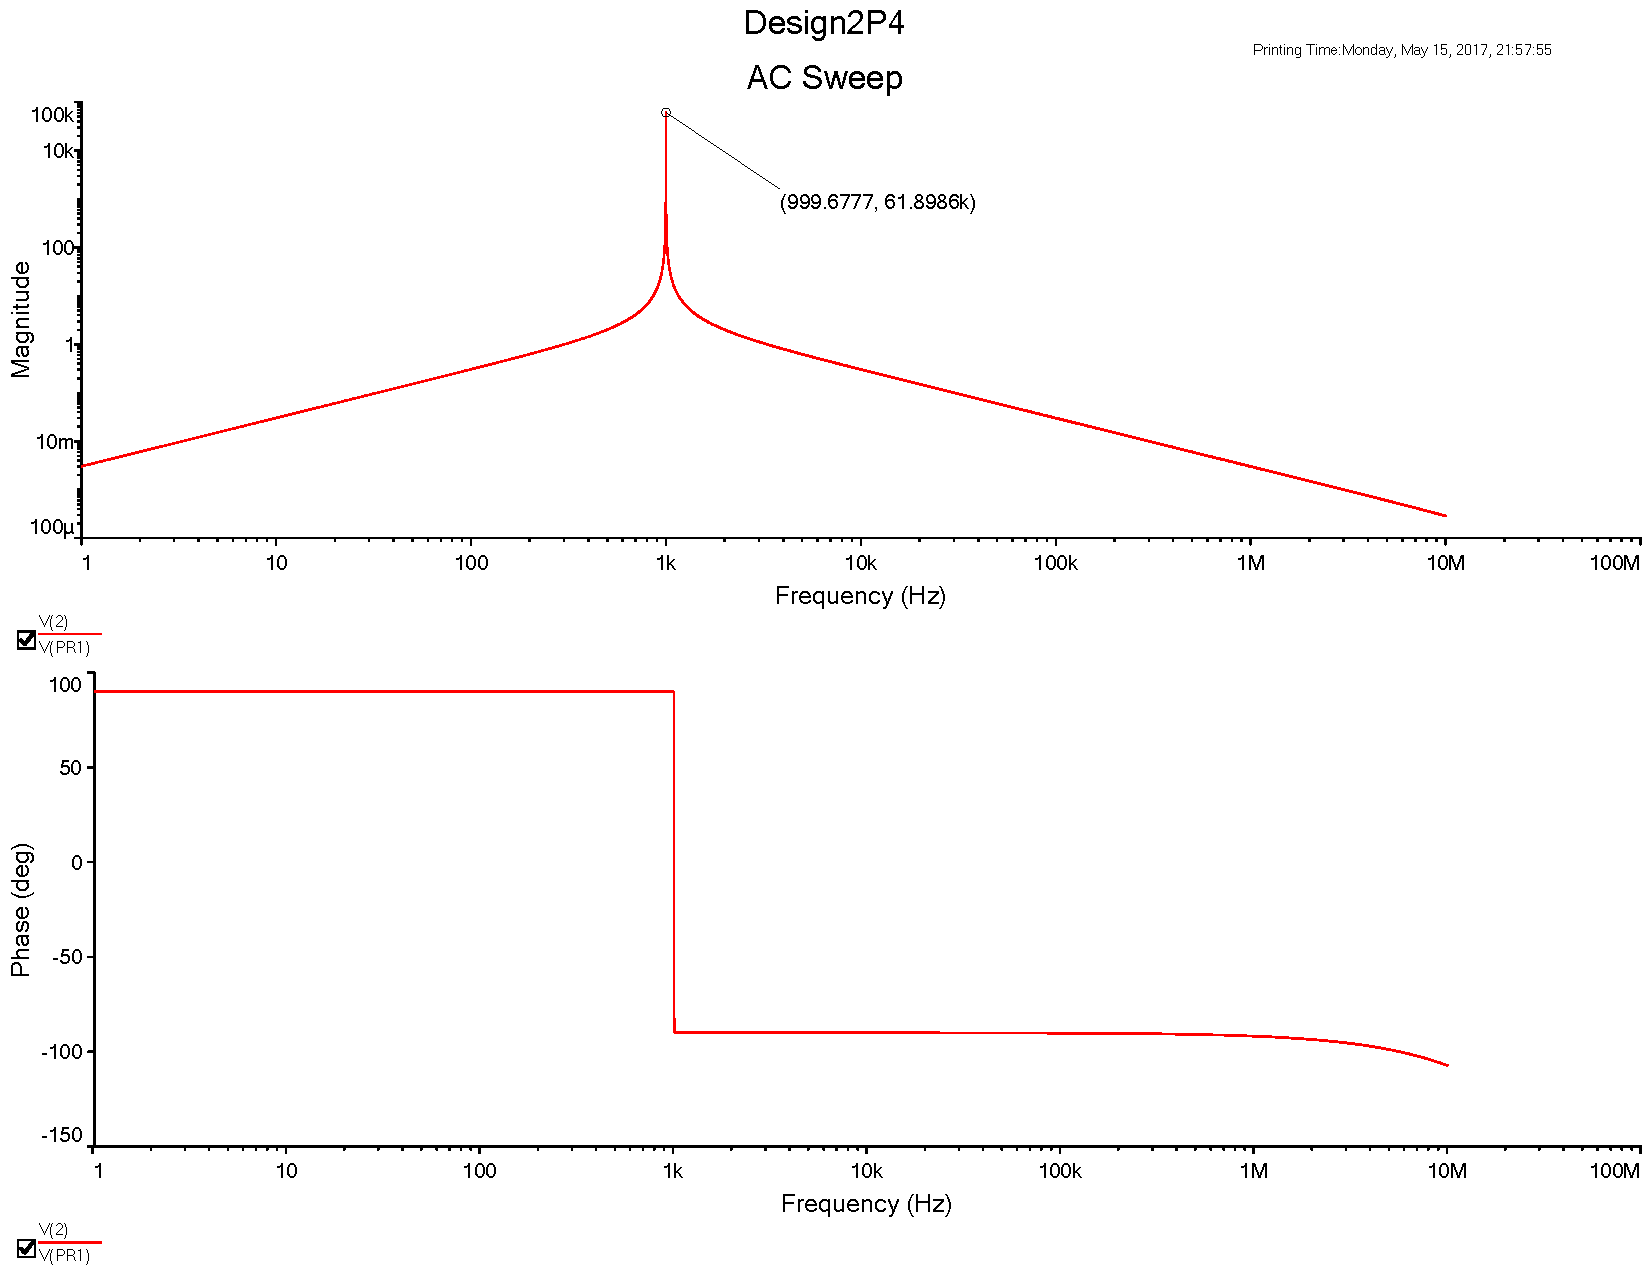
\includegraphics[width=\textwidth]{2Pinf.pdf}
\caption{$Q=\inf$}
\label{PQinf}
\end{figure}
\begin{figure}
\centering
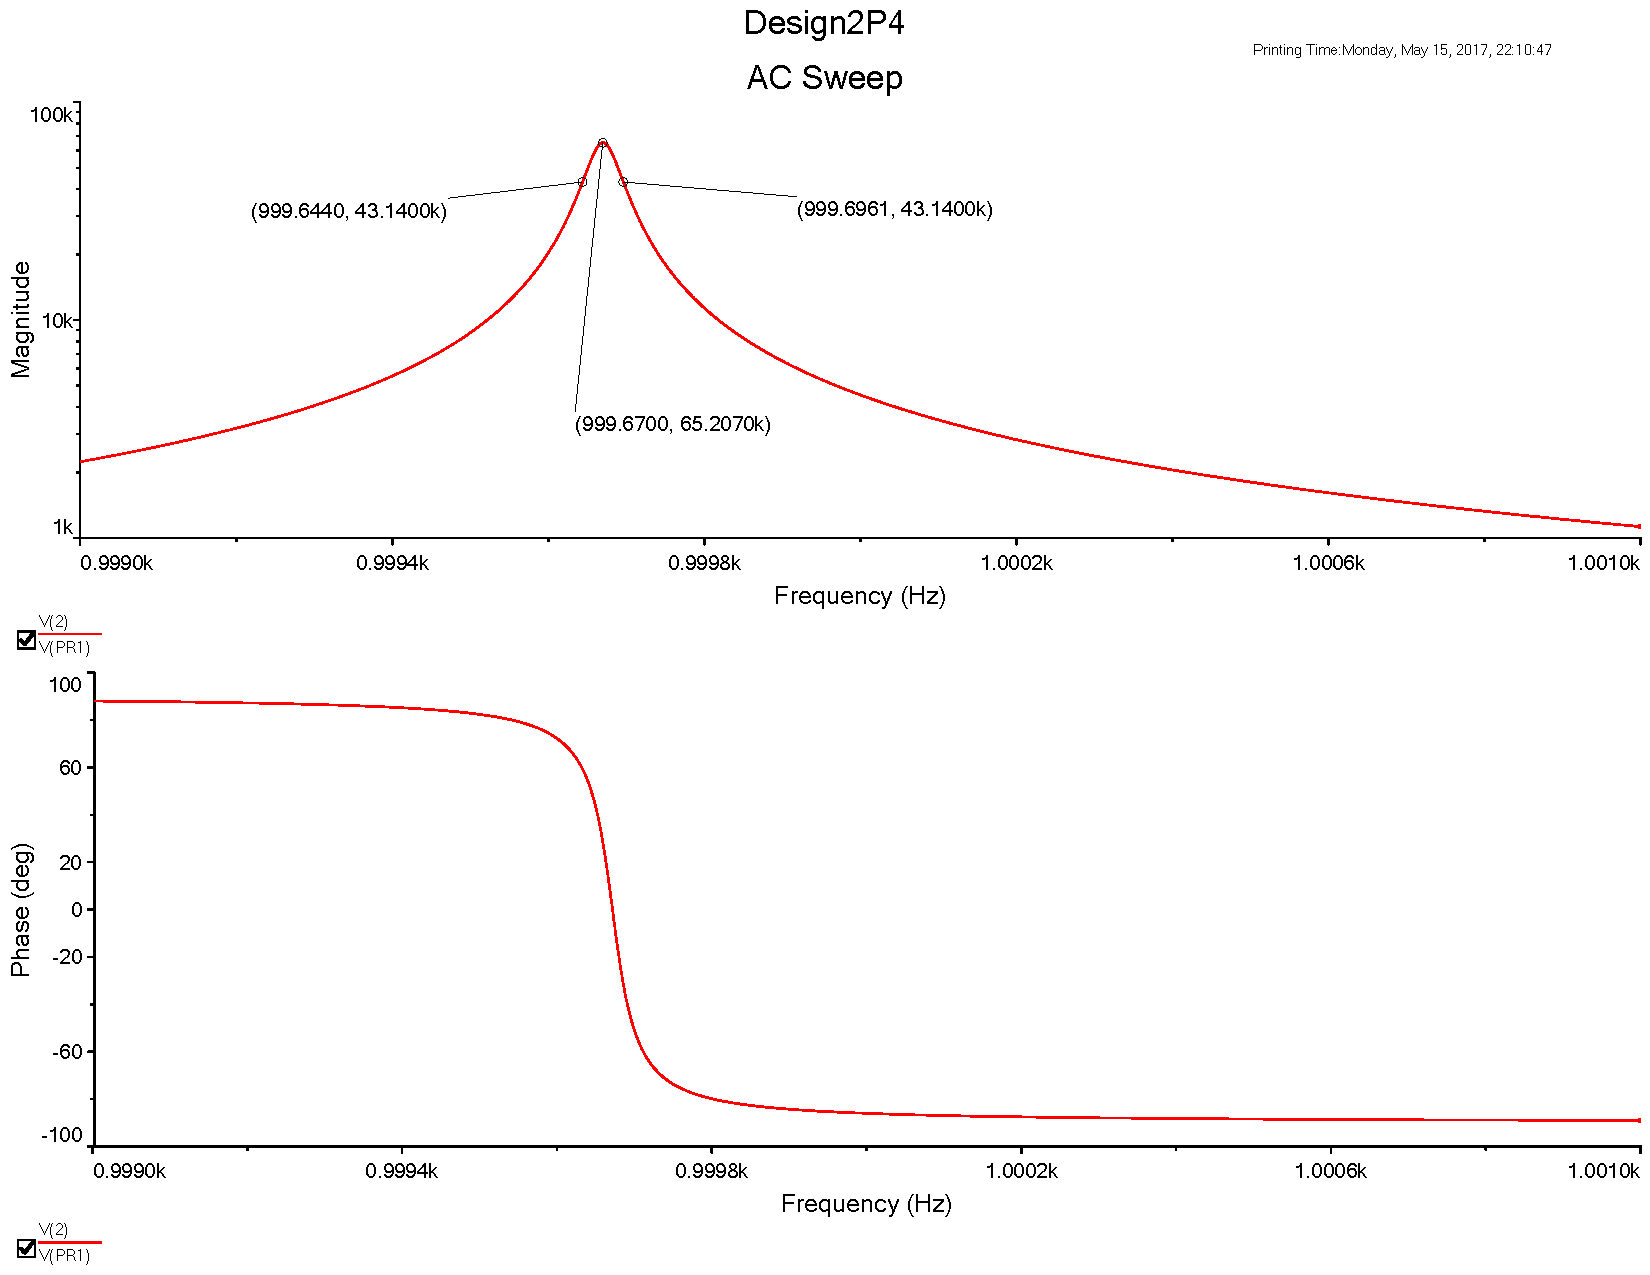
\includegraphics[width=\textwidth]{2Pinf_1.pdf}
\caption{$Q=\inf$}
\label{PQinf1}
\end{figure}
\subsubsection{倒T型网络带阻滤波器搭建和测试}
\begin{figure}
\centering
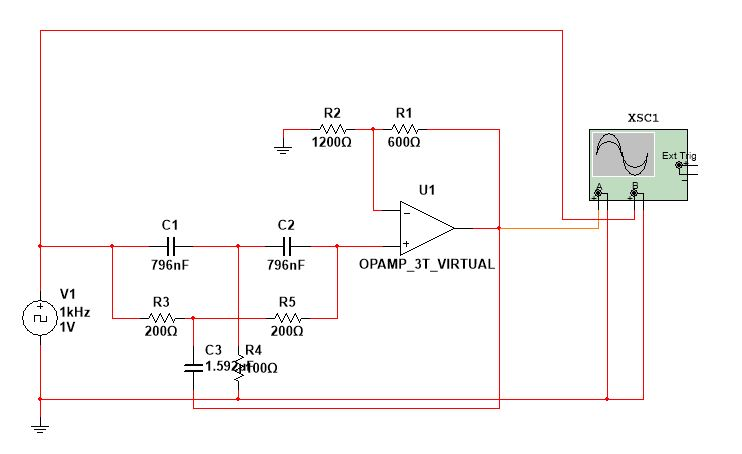
\includegraphics[width=\textwidth]{S.jpg}
\caption{倒T型网络带阻滤波器}
\label{P}
\end{figure}
\begin{figure}
\centering
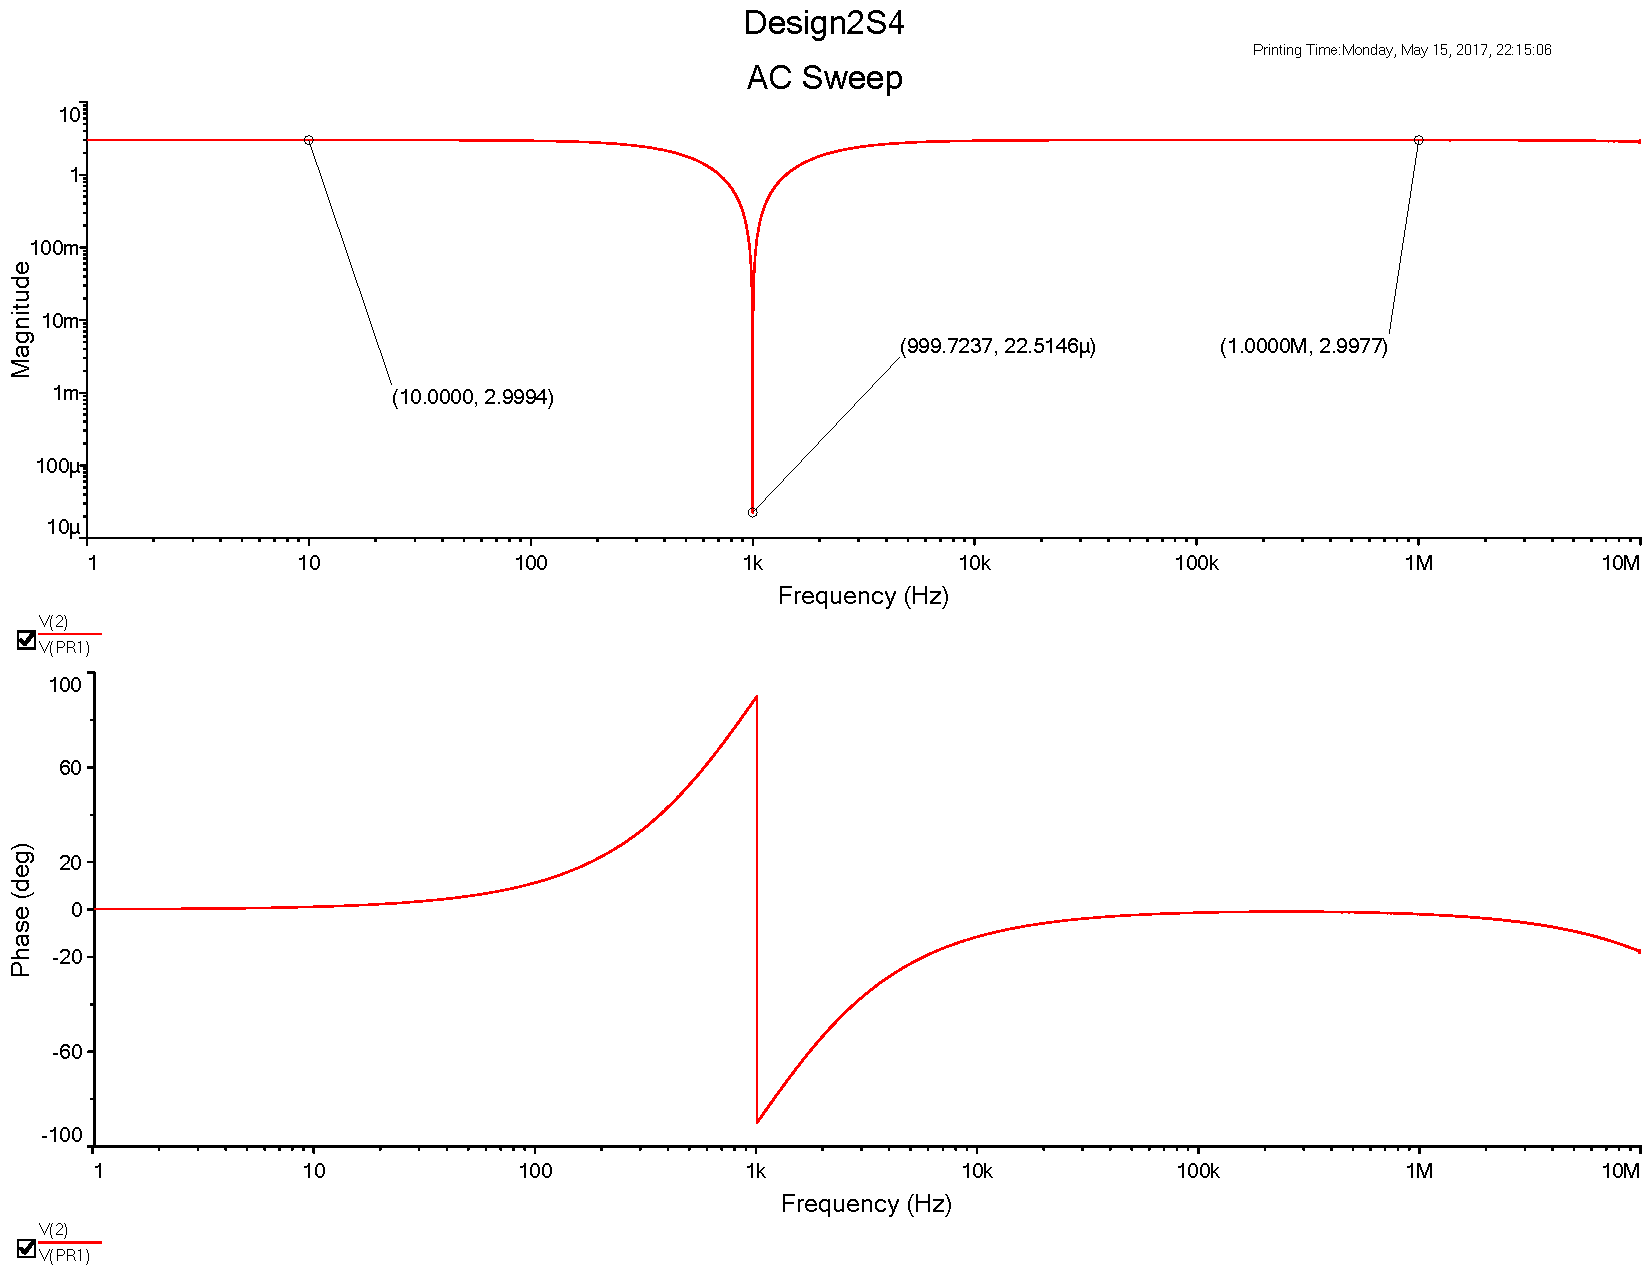
\includegraphics[width=\textwidth]{2Sinf.pdf}
\caption{倒T型网络带阻滤波器}
\label{SQ}
\end{figure}
\begin{figure}
\centering
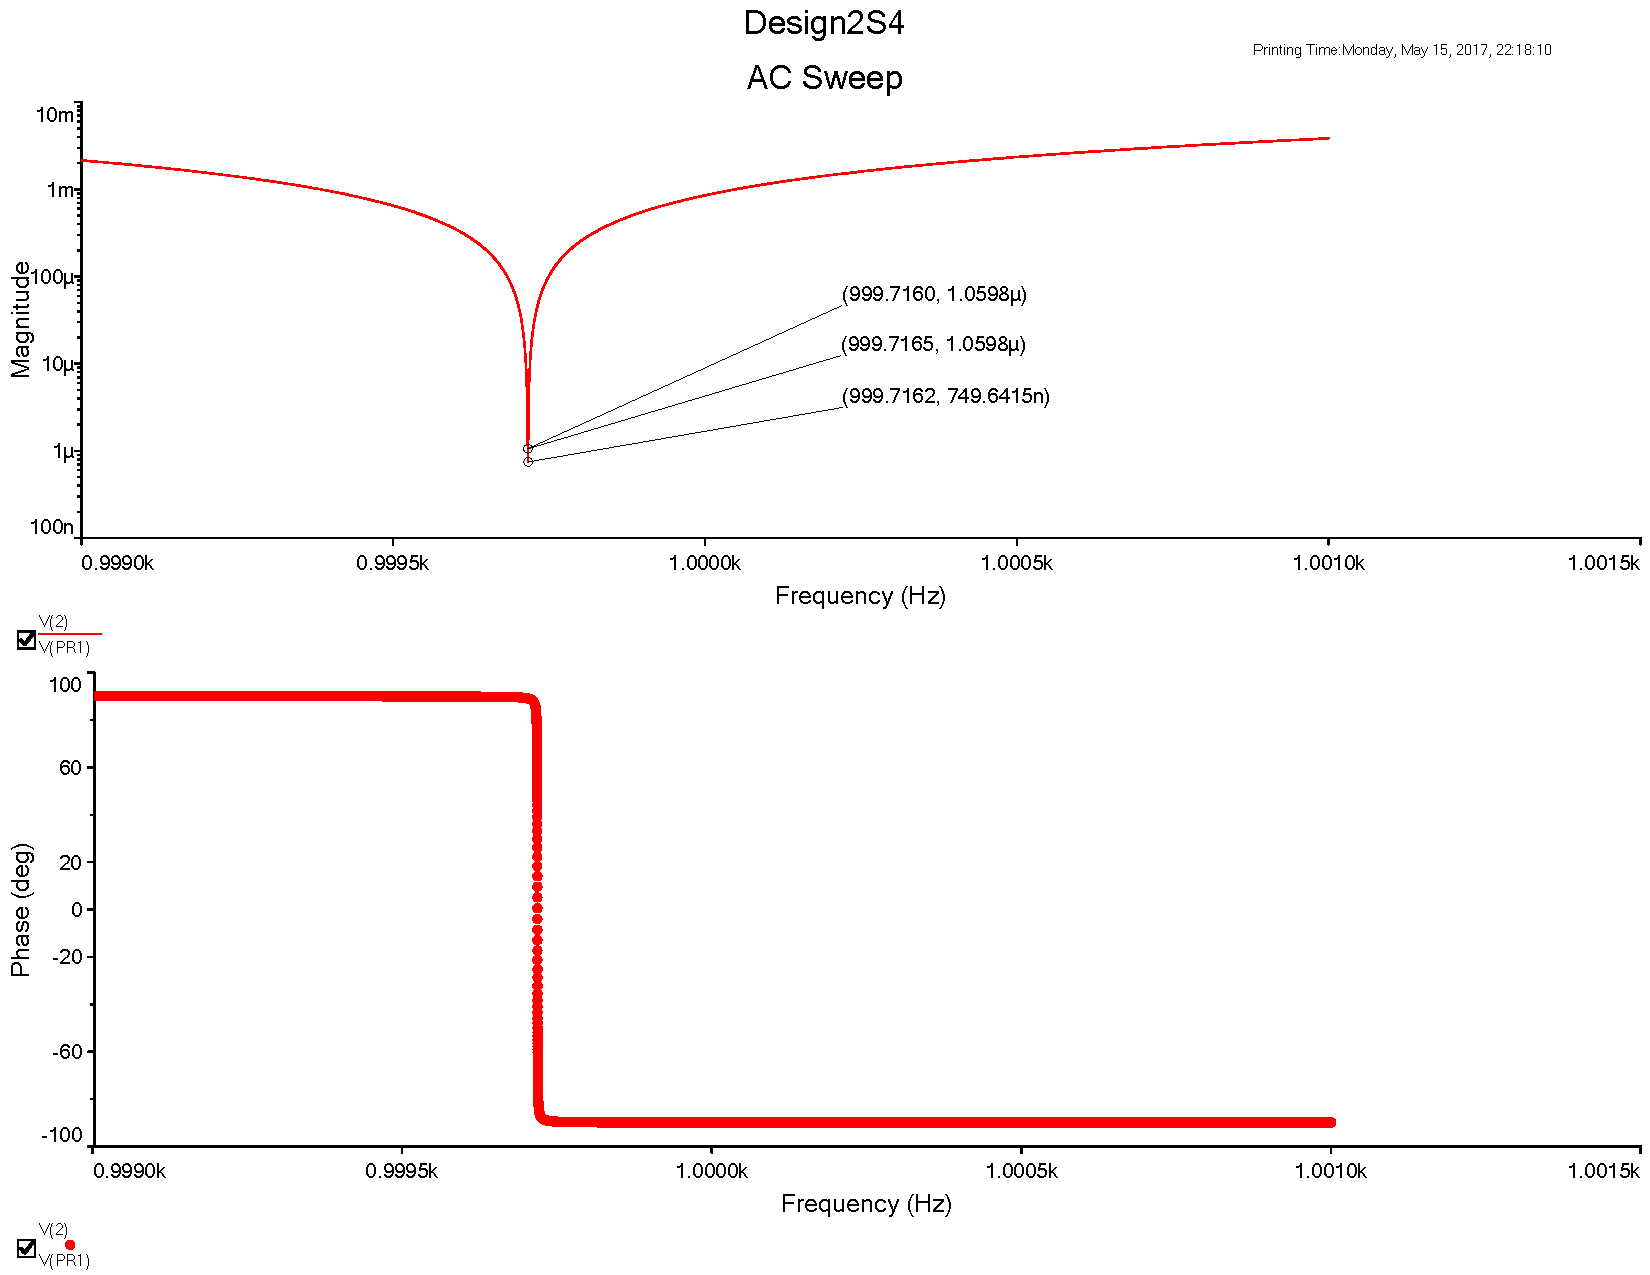
\includegraphics[width=\textwidth]{2Sinf_1.pdf}
\caption{倒T型网络带阻滤波器}
\label{SQ1}
\end{figure}
\subsection{输出波形的研究}
\subsubsection{低通滤波器波形研究}
\begin{figure}
\centering
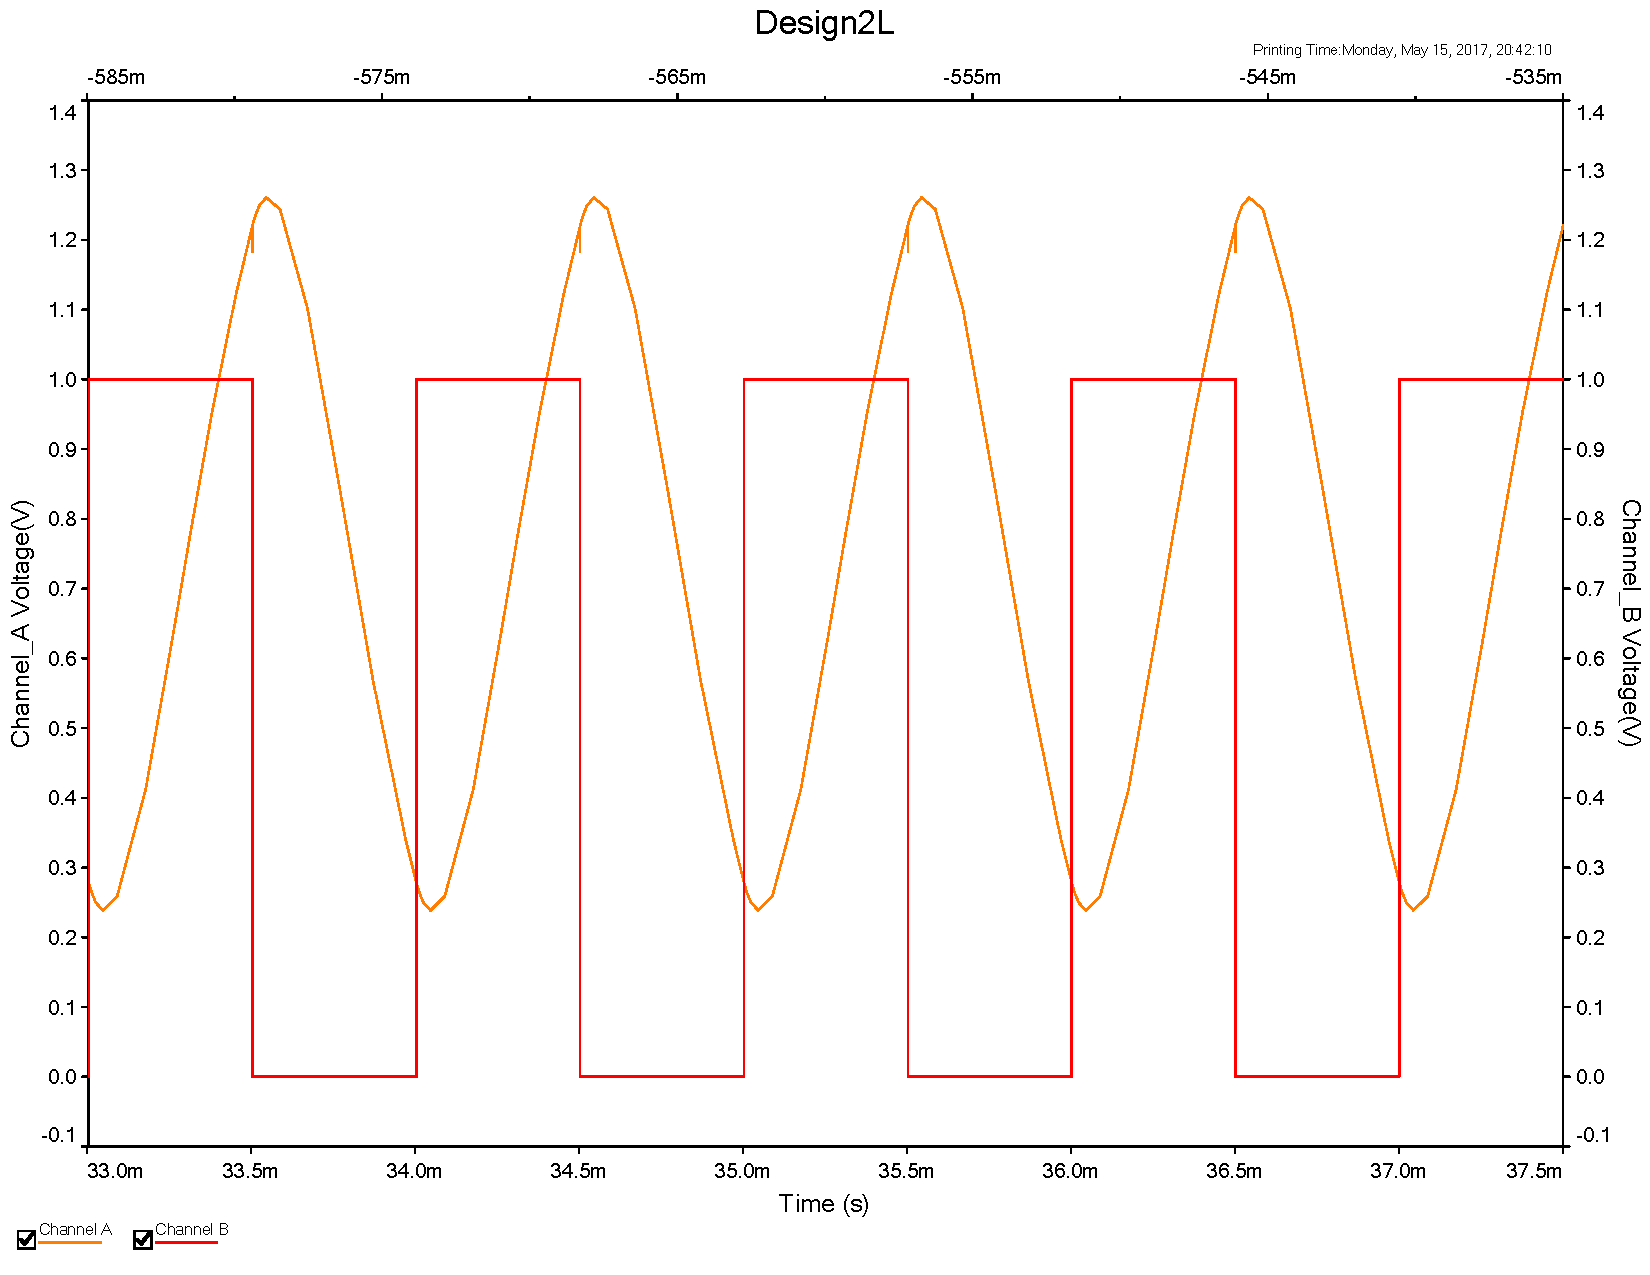
\includegraphics[width=\textwidth]{2L.pdf}
\caption{方波通过低通滤波器的波形}
\label{BIL}
\end{figure}
\subsubsection{高通滤波器波形研究}
\begin{figure}
\centering
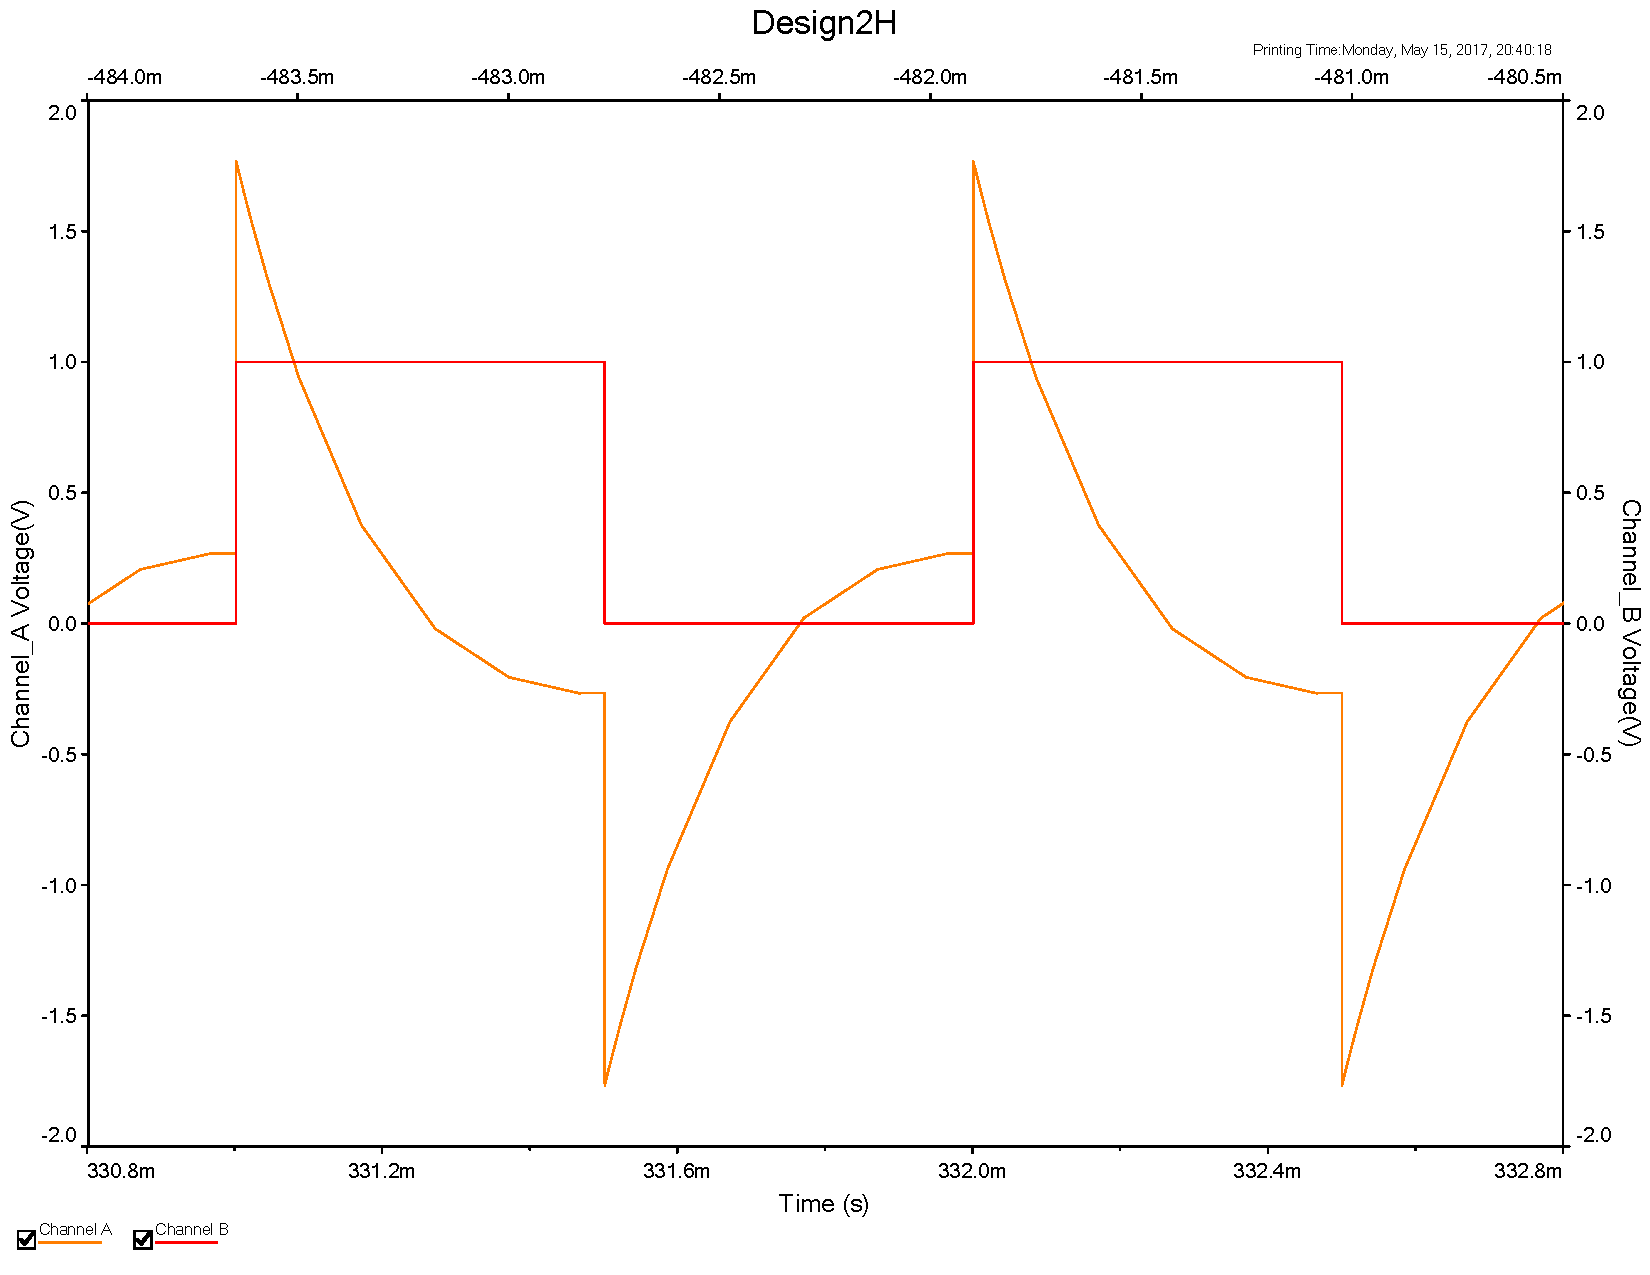
\includegraphics[width=\textwidth]{2H.pdf}
\caption{方波通过高通滤波器的波形}
\label{BIH}
\end{figure}
\subsubsection{带通滤波器波形研究}
\begin{figure}
\centering
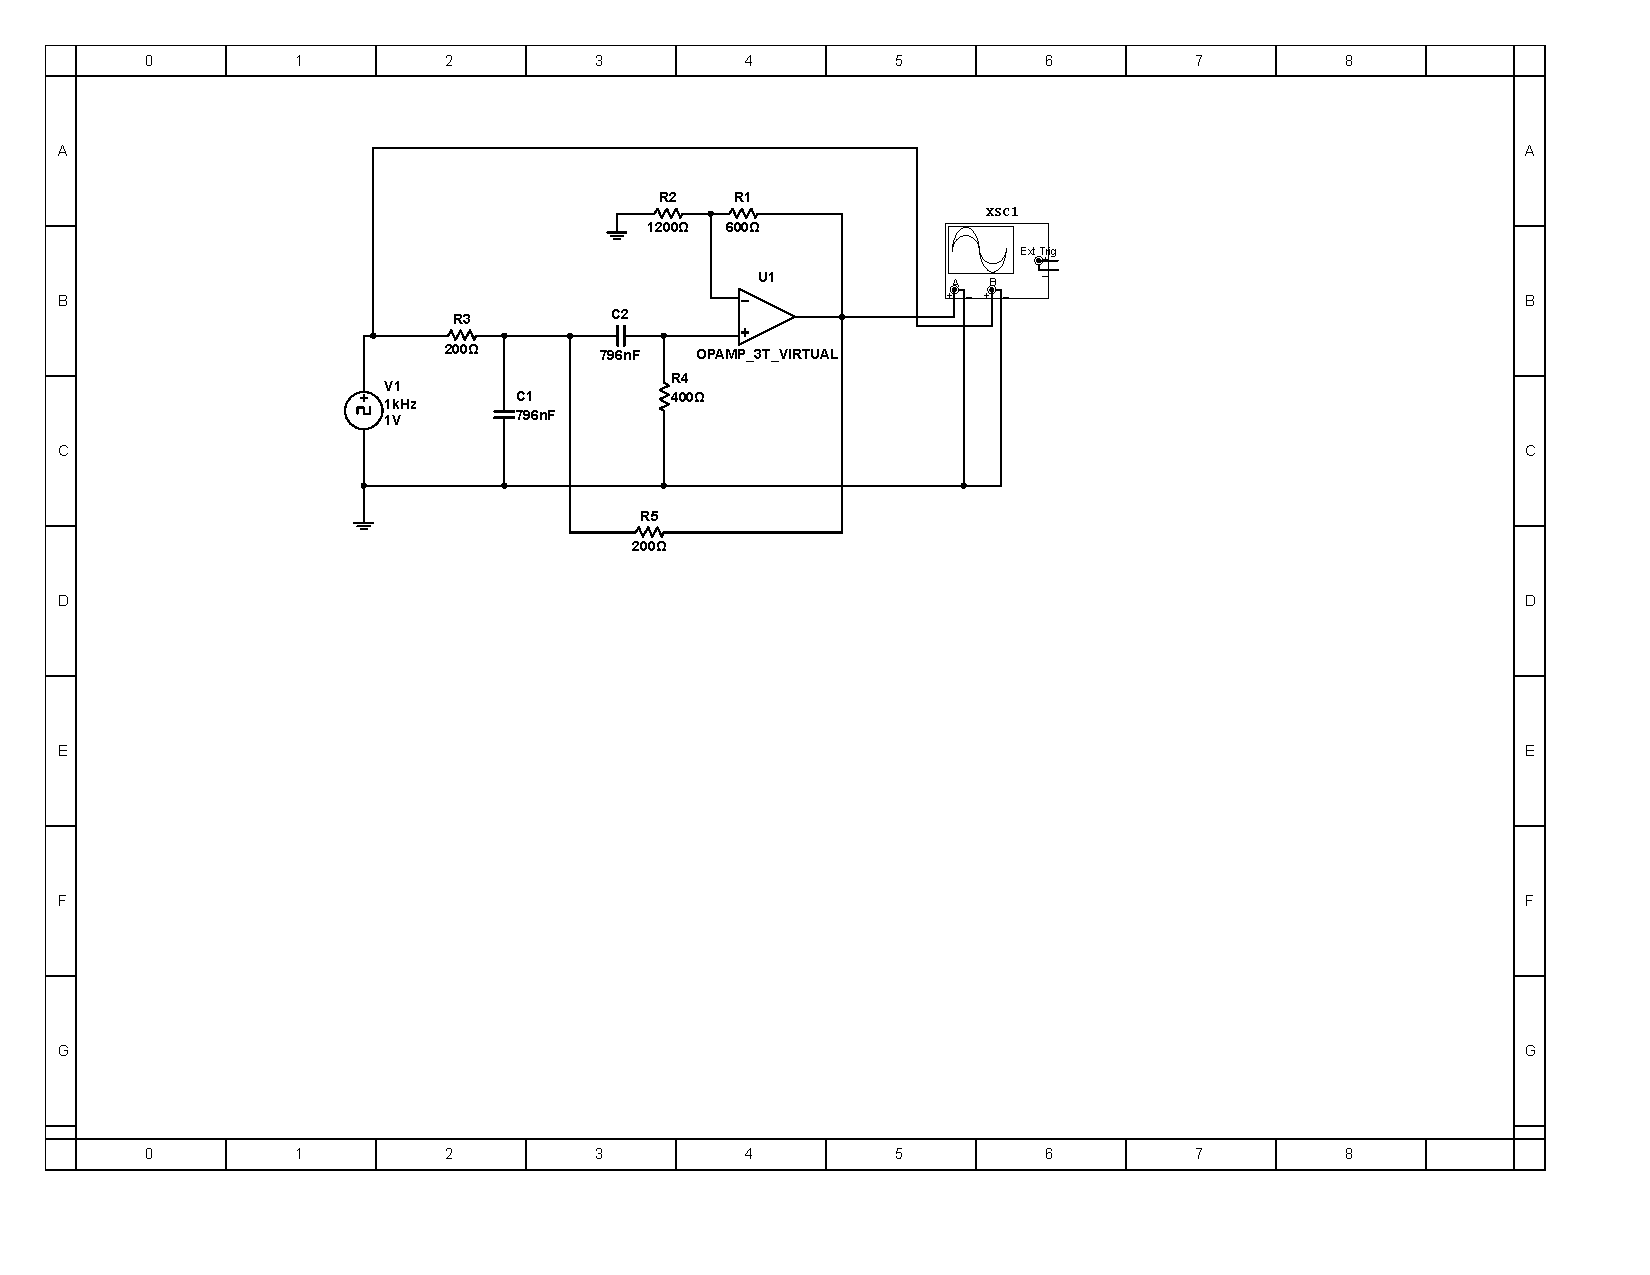
\includegraphics[width=\textwidth]{2P.pdf}
\caption{方波通过带通滤波器的波形}
\label{BIP}
\end{figure}
\subsubsection{带阻滤波器波形研究}
\begin{figure}
\centering
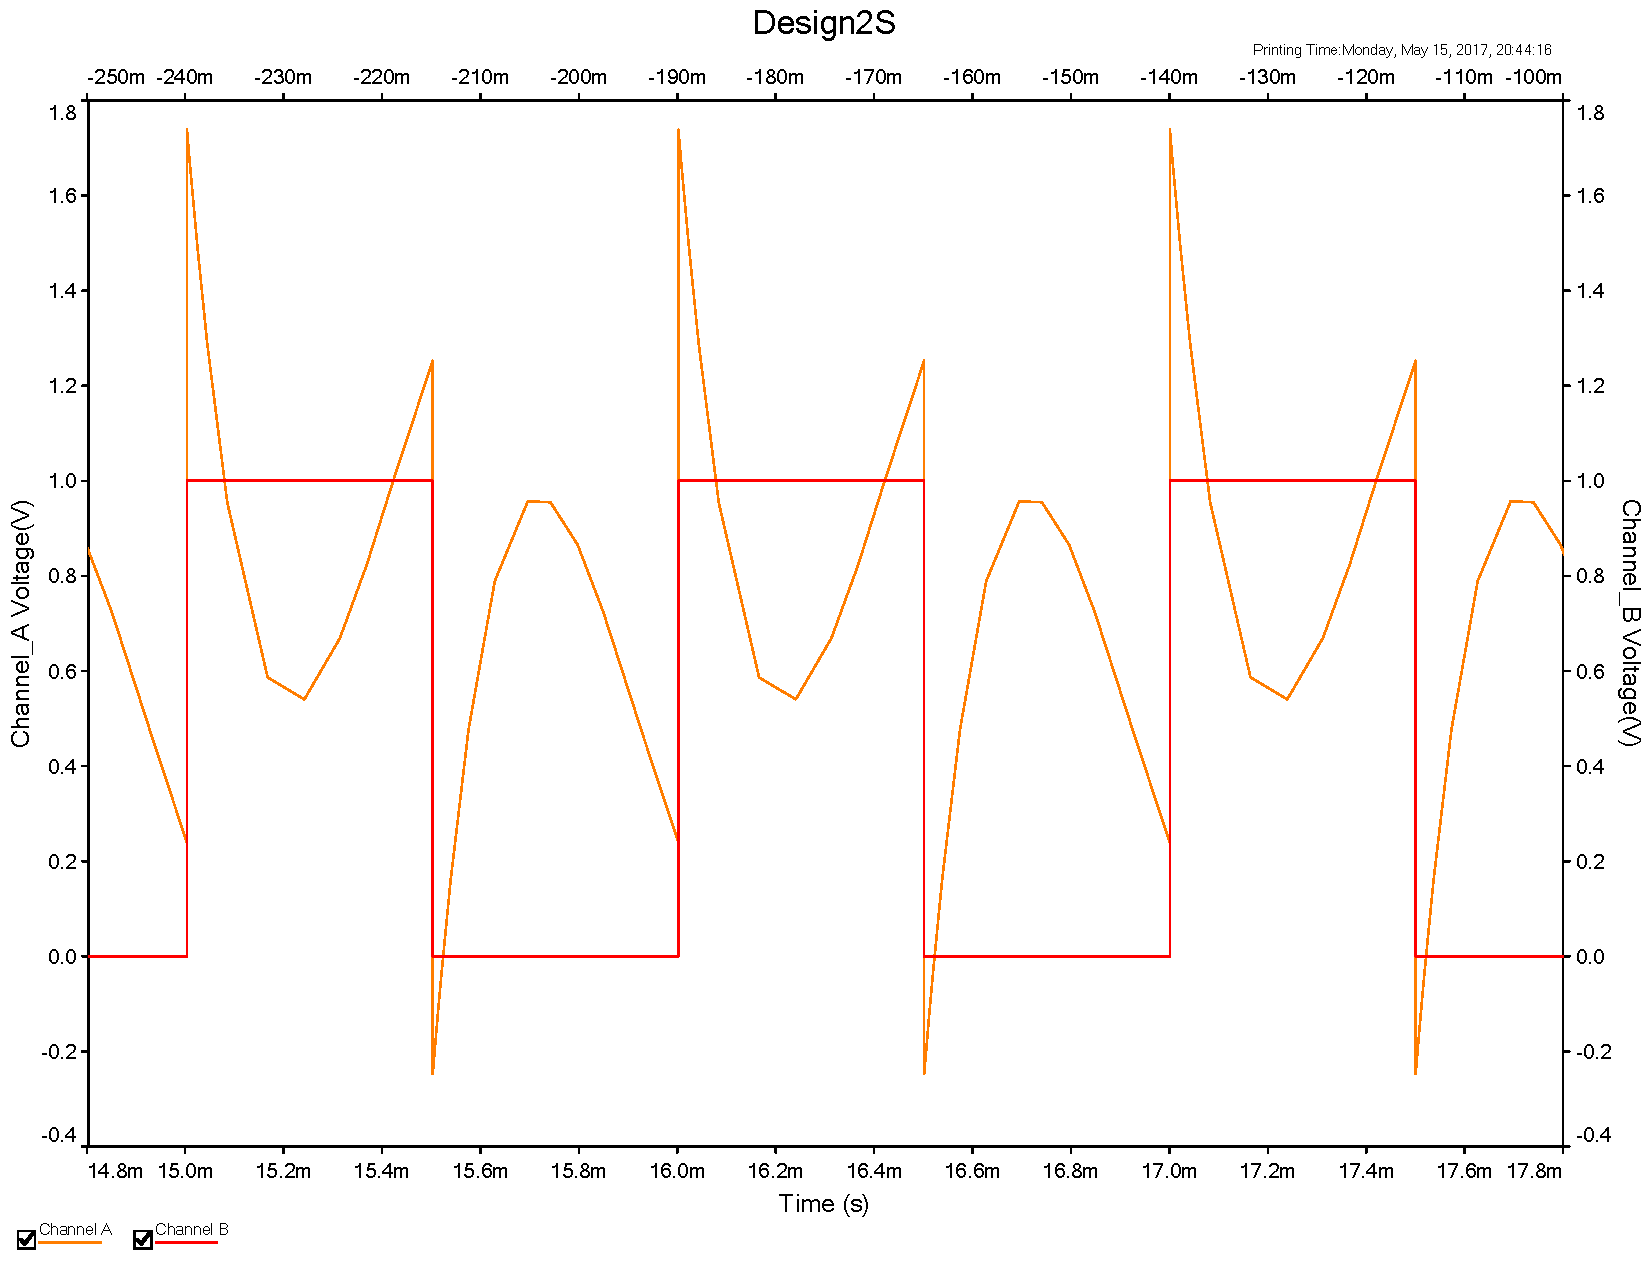
\includegraphics[width=\textwidth]{2S.pdf}
\caption{带阻通过低通滤波器的波形}
\label{BIS}
\end{figure}
\section{波形变换电路(习题7.29)}
\begin{figure}
\centering
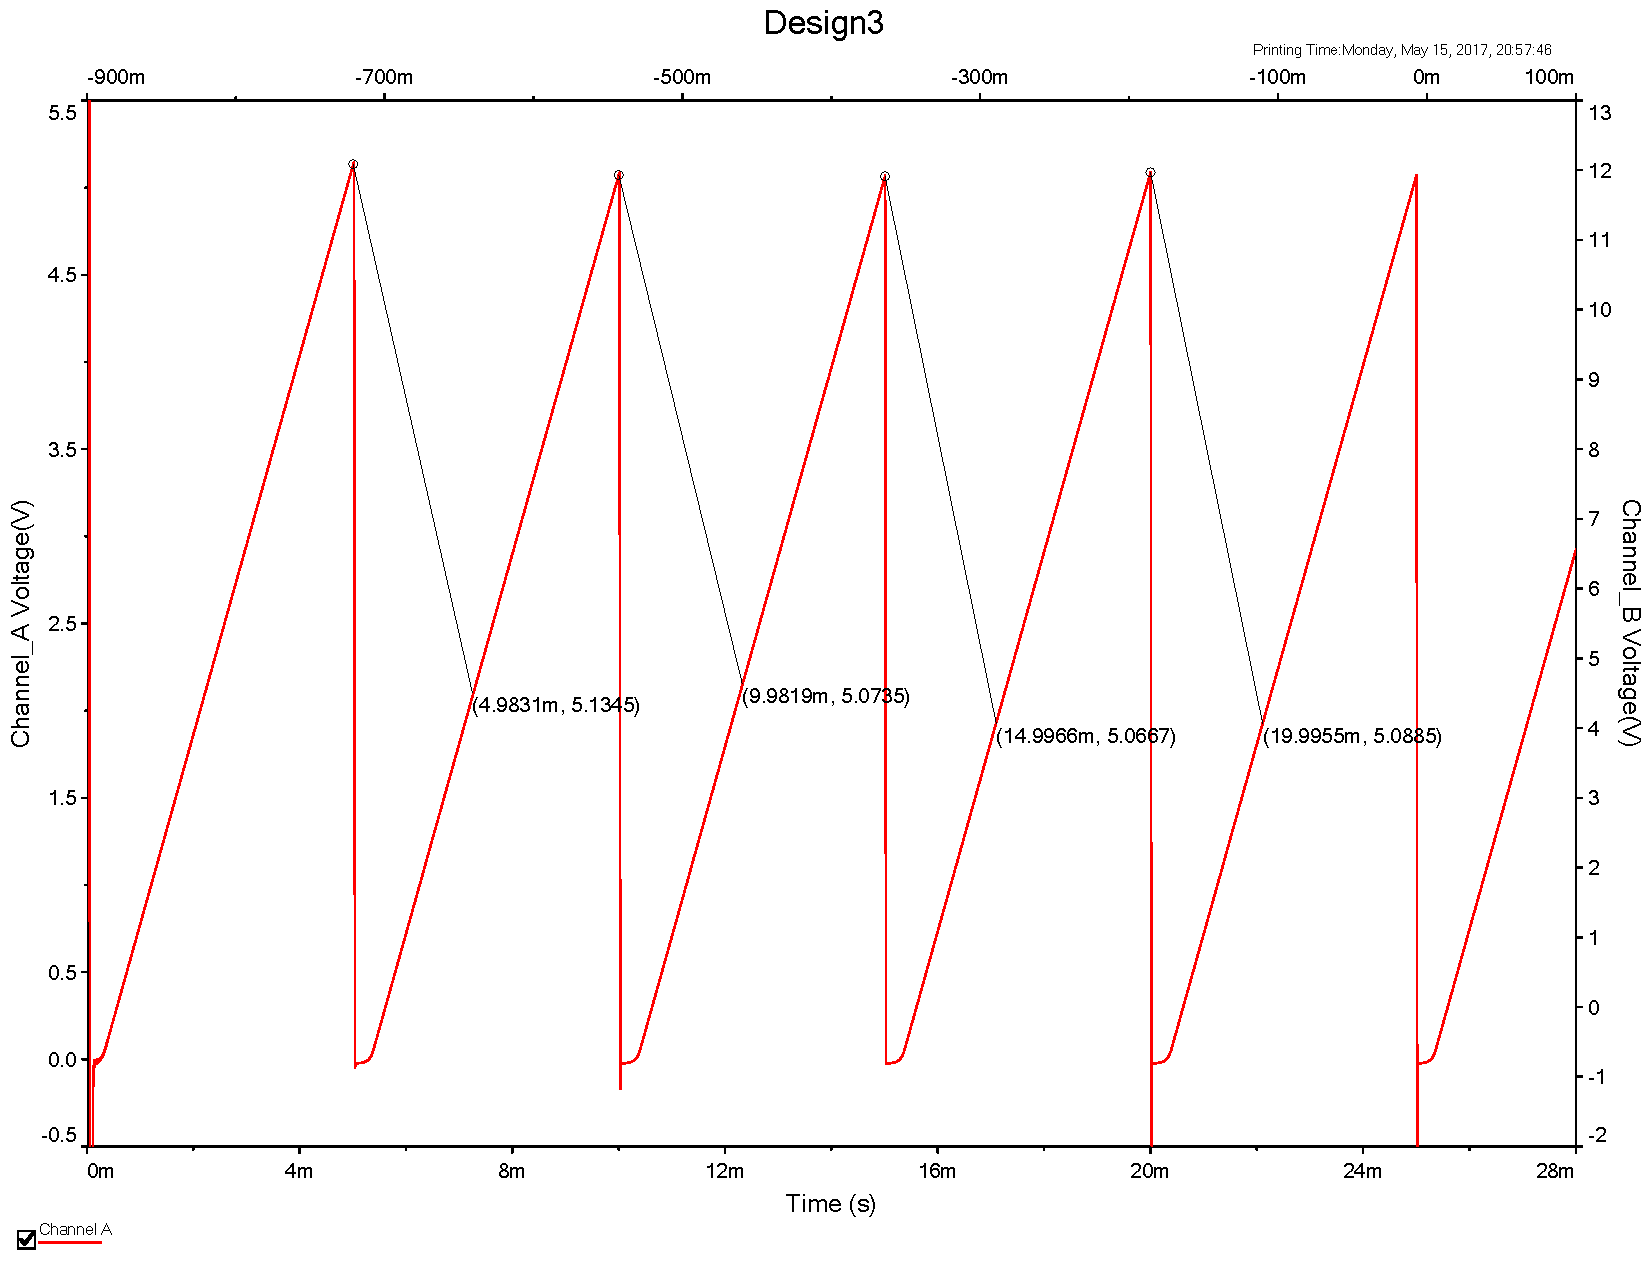
\includegraphics[width=\textwidth]{wave3.pdf}
\caption{波形}
\label{wave3}
\end{figure}

\end{document}